\documentclass[a4paper]{book}
\usepackage{makeidx}
\usepackage{natbib}
\usepackage{graphicx}
\usepackage{multicol}
\usepackage{float}
\usepackage{listings}
\usepackage{color}
\usepackage{ifthen}
\usepackage[table]{xcolor}
\usepackage{textcomp}
\usepackage{alltt}
\usepackage{ifpdf}
\ifpdf
\usepackage[pdftex,
            pagebackref=true,
            colorlinks=true,
            linkcolor=blue,
            unicode
           ]{hyperref}
\else
\usepackage[ps2pdf,
            pagebackref=true,
            colorlinks=true,
            linkcolor=blue,
            unicode
           ]{hyperref}
\usepackage{pspicture}
\fi
\usepackage[utf8]{inputenc}
\usepackage{mathptmx}
\usepackage[scaled=.90]{helvet}
\usepackage{courier}
\usepackage{sectsty}
\usepackage[titles]{tocloft}
\usepackage{doxygen}
\lstset{language=C++,inputencoding=utf8,basicstyle=\footnotesize,breaklines=true,breakatwhitespace=true,tabsize=8,numbers=left }
\makeindex
\setcounter{tocdepth}{3}
\renewcommand{\footrulewidth}{0.4pt}
\renewcommand{\familydefault}{\sfdefault}
\hfuzz=15pt
\setlength{\emergencystretch}{15pt}
\hbadness=750
\tolerance=750
\begin{document}
\hypersetup{pageanchor=false,citecolor=blue}
\begin{titlepage}
\vspace*{7cm}
\begin{center}
{\Large \-Homework 2 \-Design \-Document }\\
\vspace*{1cm}
{\large \-Generated by Doxygen 1.7.6.1}\\
\vspace*{0.5cm}
{\small Sun Oct 14 2012 17:01:03}\\
\end{center}
\end{titlepage}
\clearemptydoublepage
\pagenumbering{roman}
\tableofcontents
\clearemptydoublepage
\pagenumbering{arabic}
\hypersetup{pageanchor=true,citecolor=blue}
\chapter{\-Homework 2 \-Design \-Document\-: \-Snake 2.0 \-Game using \-Q\-T \-Library}
\label{index}\hypertarget{index}{}\begin{DoxyAuthor}{\-Author}
\-Chad \-Martin
\end{DoxyAuthor}


 \hypertarget{index_Overview}{}\section{\-Purpose/\-Overview}\label{index_Overview}
\-The program starts out by displaying intro screen 1 which asks the user for a number from 1 to 5 which correlates to the speed of the snake and the points multiplier. 1 is the slowest speed and 5 is the fastest speed. \-The faster the speed the bigger the points multiplier. 

\-Next intro screen 2 is displayed, the user is asked if he/she would like to enable wrap around. \-If wrap around is enabled, the snake is allowed to go through the borders. \-If wrap around is disabled and the snake hits the borders, it will cause a game over. \-Also, \-If wrap around is disabled, the points multiplier is doubled. 

\-After the game options are set, the game starts at 0 points with 2 pieces on the screen. \-One of the pieces is a \hyperlink{classSnakeBlock}{\-Snake\-Block} head. \-This piece is the snake that the user controls with the arrow keys. \-The other piece is a green \-Apple logo. \-This piece is a normal piece of food. \-When the snake collides with the normal piece of food, the snake will grow 1 block and the points will increase by 7 times the points multiplier. \-After the collision, the food will spawn in a new random location. \-Also in the window, there is an i\-Phone. \-This is the border around the screen. \-On the status bar of the i\-Phone, the points that the user has accumulated are displayed. \-If the snake head runs over another part of the snake, it will always cause a game over. \-If wrap around is disabled and the snake hits the border, it will cause a game over. 

\-Another piece that can spawn is a \-Windows 8 logo. \-This piece is a special piece of food. \-When the snake collides with the special piece of food, the game will go into a blue screen of death. \-This piece will spawn every ten grows or if ‘\-W’ is pressed. 

\-Another piece that can spawn is a \-Linux logo. \-This piece is the winning piece of food. \-When the snake collides with the winning piece of food, the game will end and a victory screen will appear. \-This piece will spawn after the special piece of food is painted in 100 paint events or if ‘\-L’ is pressed. 

\-When a blue screen of death occurs, the game stops, the users points are set to zero, and a blue screen of death is displayed. \-After any key is pressed the game moves on to the game over screen. 

\-When a game over occurs, the game stops and the game over screen is displayed. \-On the game over screen, the words game over, the total number of points, and instructions for the user to play again are displayed. \-If the user presses the \-Space bar, the game starts over and intro screen 1 is displayed. 

\-When a victory occurs, the game stops and the victory screen is displayed. \-On the victory screen, the words victory, the total number of points, and instructions for the user to play again are displayed. \-If the user presses the \-Space bar, the game starts over and intro screen 1 is displayed. 

\-If the user presses \-E\-S\-C at any time during the program, the program will quit.



 \hypertarget{index_Requirements}{}\section{\-Requirements}\label{index_Requirements}
\-Entertain the user through playing the game. \-Find the \-Linux logo and eat it to win the game.



 \hypertarget{index_Instructions}{}\section{\-Instructions}\label{index_Instructions}
\-In order to compile this program,
\begin{DoxyItemize}
\item extract files from \-Chad\-Mart\-\_\-\-H\-W2.\-zip
\item navigate to the `/hw2/ directory
\item enter “qmake -\/project” in terminal
\item enter “qmake” in terminal
\item enter “make” in terminal
\end{DoxyItemize}

\-In order to run this program,
\begin{DoxyItemize}
\item enter “./hw2” in terminal
\end{DoxyItemize}

\-Program library dependencies
\begin{DoxyItemize}
\item \-Q\-T library
\begin{DoxyItemize}
\item $<$\-Q\-Desktop\-Widget$>$
\item $<$\-Q\-Application$>$
\item $<$\-Q\-Widget$>$
\item $<$\-Q\-Key\-Event$>$
\item $<$\-Q\-Image$>$
\item $<$\-Q\-Rect$>$
\item $<$\-Q\-Painter$>$
\end{DoxyItemize}
\item \-C \-Standard \-General \-Utilities \-Library
\begin{DoxyItemize}
\item $<$stdlib.\-h$>$
\end{DoxyItemize}
\item vector \-Library
\begin{DoxyItemize}
\item $<$vector$>$
\end{DoxyItemize}
\end{DoxyItemize}



 \hypertarget{index_Classes}{}\section{\-Classes}\label{index_Classes}

\begin{DoxyItemize}
\item \hyperlink{classGame}{\-Game}
\item \hyperlink{classSnake}{\-Snake}
\item \hyperlink{classSnakeBlock}{\-Snake\-Block}
\item \hyperlink{classFood}{\-Food}
\begin{DoxyItemize}
\item \hyperlink{classSpecialFood}{\-Special\-Food}
\item \hyperlink{classFoodWinner}{\-Food\-Winner}
\end{DoxyItemize}
\item \hyperlink{classIphone}{\-Iphone}
\end{DoxyItemize}



 \hypertarget{index_Global_functions}{}\section{\-Global Data/\-Functions}\label{index_Global_functions}

\begin{DoxyItemize}
\item \-Global \-Functions
\begin{DoxyItemize}
\item void center (\-Q\-Widget \&widget)
\begin{DoxyItemize}
\item \-Sets up window size and centers window on screen.
\item \-Precondition\-: \-Program has started.
\item \-Postcondition\-: \hyperlink{classGame}{\-Game} window is displayed on center of screen.
\end{DoxyItemize}
\end{DoxyItemize}
\end{DoxyItemize}



 \hypertarget{index_High-level_Architecture}{}\section{\-High-\/level Architecture}\label{index_High-level_Architecture}
\-When the program starts, the \-Q\-T window is initialized and the basic window settings are set such as the size of the window. \-Then \hyperlink{classGame}{\-Game} is launched. \-Next, the required objects are created from the following classes\-: \hyperlink{classSnake}{\-Snake}, \hyperlink{classFood}{\-Food}, \hyperlink{classSpecialFood}{\-Special\-Food}, \-Winning\-Food, and i\-Phone. \-When an object of the \hyperlink{classSnake}{\-Snake} class is created, a vector of \hyperlink{classSnakeBlock}{\-Snake\-Block} objects is created. \-After that, the paint event is called which displays intro screen 1. \-The user is asked to select the speed which will set the timer delay and the points multiplier. \-Once the user makes a selection, another paint event is called which displays intro screen 2. \-During intro screen 2, the user is asked to whether to enable or disable wrap around which will set wraparound to \-T\-R\-U\-E or \-F\-A\-L\-S\-E. \-Once the user makes a selection, start\-Game is called which starts the timer, resets data members to default values, deletes \hyperlink{classSnake}{\-Snake}, creates a new \hyperlink{classSnake}{\-Snake} dynamically, and moves food using move\-Food and check\-Bad\-Food methods of the \hyperlink{classFood}{\-Food} class. \-Then, another paint event is called which displays the game play screen. 

\-Now, the game begins. \-Once the user presses an arrow key, the snake begins to move by the auto\-Move method of the \hyperlink{classSnake}{\-Snake} class and collision detection occurs after each time the snake moves by the check\-Collision method of the game class. \-If during check\-Collision the snake makes an illegal collision, then the game\-Over function is called and the game either restarts or the program terminates. \-If during check\-Collision the snake collides with an \-Apple logo, the snake grows 1 \hyperlink{classSnakeBlock}{\-Snake\-Block} using snake-\/$>$grow and points are added to points. \-If during check\-Collision the snake collides with a \-Windows 8 logo, the blue\-Screen\-Death function is called which displays the bsod. \-If during check\-Collision the snake collides with a \-Linux logo, the victory screen is displayed using the victory function. \-If the user presses ‘\-P’, pause\-Game function is called and game is paused. 

\-If the user presses \-E\-S\-C at any time, q\-App-\/$>$exit function is called and program is terminated. 

\-If the user presses ‘\-R’ at any time, stop\-Game function is called, intro\-Prompt1 is set to true, and intro screen 1 is displayed.



 \hypertarget{index_UI}{}\section{\-User Interface}\label{index_UI}
\-Universal \-Controls
\begin{DoxyItemize}
\item \-Esc key is pressed
\begin{DoxyItemize}
\item \-Exits app
\end{DoxyItemize}
\item '\-R' key is pressed
\begin{DoxyItemize}
\item \hyperlink{classGame}{\-Game} is reset
\item \-Intro \-Screen 1 is displayed
\end{DoxyItemize}
\end{DoxyItemize}

\-Intro \-Screen 1 

\-Intro \-Screen 1 \-Controls
\begin{DoxyItemize}
\item '1' key is pressed
\begin{DoxyItemize}
\item point\-Multi = 1;
\item speed\-Delay = 200;
\item \-Intro \-Screen 2 is displayed
\end{DoxyItemize}
\item '2' key is pressed
\begin{DoxyItemize}
\item point\-Multi = 2;
\item speed\-Delay = 169;
\item \-Intro \-Screen 2 is displayed
\end{DoxyItemize}
\item '3' key is pressed
\begin{DoxyItemize}
\item point\-Multi = 3;
\item speed\-Delay = 138;
\item \-Intro \-Screen 2 is displayed
\end{DoxyItemize}
\item '4' key is pressed
\begin{DoxyItemize}
\item point\-Multi = 4;
\item speed\-Delay = 107;
\item \-Intro \-Screen 2 is displayed
\end{DoxyItemize}
\item '5' key is pressed
\begin{DoxyItemize}
\item point\-Multi = 5;
\item speed\-Delay = 75;
\item \-Intro \-Screen 2 is displayed
\end{DoxyItemize}
\item '9' key is pressed
\begin{DoxyItemize}
\item point\-Multi = 1000;
\item speed\-Delay = 0;
\item \-Intro \-Screen 2 is displayed
\end{DoxyItemize}
\end{DoxyItemize}

\-Intro \-Screen 2 

\-Intro \-Screen 2 \-Controls
\begin{DoxyItemize}
\item '\-Y' key is pressed
\begin{DoxyItemize}
\item wrap\-Around = \-T\-R\-U\-E;
\item \hyperlink{classGame}{\-Game} is started
\end{DoxyItemize}
\item '\-N' key is pressed
\begin{DoxyItemize}
\item wrap\-Around = \-F\-A\-L\-S\-E;
\item \hyperlink{classGame}{\-Game} is started
\end{DoxyItemize}
\end{DoxyItemize}

\hyperlink{classGame}{\-Game} \-Over \-Screen 

\hyperlink{classGame}{\-Game} \-Over \-Screen \-Controls
\begin{DoxyItemize}
\item \-Space bar
\begin{DoxyItemize}
\item \-Intro \-Screen 1 is displayed
\end{DoxyItemize}
\end{DoxyItemize}

\-Victory \-Screen 

\-Victory \-Screen \-Controls
\begin{DoxyItemize}
\item \-Space bar is pressed
\begin{DoxyItemize}
\item \-Intro \-Screen 1 is displayed
\end{DoxyItemize}
\end{DoxyItemize}

\-Blue \-Screen of \-Death 

\-Blue \-Screen of \-Death \-Controls
\begin{DoxyItemize}
\item \-Any key is pressed, expect '\-R' or \-E\-S\-C
\begin{DoxyItemize}
\item \hyperlink{classGame}{\-Game} \-Over \-Screen is displayed
\end{DoxyItemize}
\end{DoxyItemize}

\hyperlink{classGame}{\-Game} \-Play \-Screen 

\hyperlink{classGame}{\-Game} \-Play \-Controls
\begin{DoxyItemize}
\item \-Normal \hyperlink{classGame}{\-Game} \-Play \-Controls
\begin{DoxyItemize}
\item \-Right arrow key is pressed
\begin{DoxyItemize}
\item \hyperlink{classSnake}{\-Snake} moves right
\end{DoxyItemize}
\item \-Left arrow key is pressed
\begin{DoxyItemize}
\item \hyperlink{classSnake}{\-Snake} moves left
\end{DoxyItemize}
\item \-Up arrow key is pressed
\begin{DoxyItemize}
\item \hyperlink{classSnake}{\-Snake} moves up
\end{DoxyItemize}
\item \-Down arrow key is pressed
\begin{DoxyItemize}
\item \hyperlink{classSnake}{\-Snake} moves down
\end{DoxyItemize}
\item '\-P' key is pressed
\begin{DoxyItemize}
\item \-Pauses game (\hyperlink{classSnake}{\-Snake} stops moving)
\end{DoxyItemize}
\end{DoxyItemize}
\item \-Paused \hyperlink{classGame}{\-Game} \-Play \-Controls
\begin{DoxyItemize}
\item \-Right arrow key is pressed
\begin{DoxyItemize}
\item \hyperlink{classGame}{\-Game} resumes
\item \hyperlink{classSnake}{\-Snake} moves right
\end{DoxyItemize}
\item \-Left arrow key is pressed
\begin{DoxyItemize}
\item \hyperlink{classGame}{\-Game} resumes
\item \hyperlink{classSnake}{\-Snake} moves left
\end{DoxyItemize}
\item \-Up arrow key is pressed
\begin{DoxyItemize}
\item \hyperlink{classGame}{\-Game} resumes
\item \hyperlink{classSnake}{\-Snake} moves up
\end{DoxyItemize}
\item \-Down arrow key is pressed
\begin{DoxyItemize}
\item \hyperlink{classGame}{\-Game} resumes
\item \hyperlink{classSnake}{\-Snake} moves down
\end{DoxyItemize}
\item '\-P' key is pressed
\begin{DoxyItemize}
\item \hyperlink{classGame}{\-Game} resumes
\item \hyperlink{classSnake}{\-Snake} moves in the last direction
\end{DoxyItemize}
\end{DoxyItemize}
\item \-Cheat \-Codes (\-Only active during \-Normal \hyperlink{classGame}{\-Game} \-Play)
\begin{DoxyItemize}
\item '\-M' key or '\-A' key is pressed
\begin{DoxyItemize}
\item switches food images
\item \-Moves the apple
\end{DoxyItemize}
\item '\-G' key is pressed
\begin{DoxyItemize}
\item \-Grows snake, but doesn't increase points
\end{DoxyItemize}
\item '\-W' key is pressed
\begin{DoxyItemize}
\item \-Moves special\-Food (the \-Windows 8 logo)
\item \-Paints special\-Food
\end{DoxyItemize}
\item '8' key is pressed
\begin{DoxyItemize}
\item \-Displays blue screen of death
\item \-Causes \-B\-S\-O\-D \hyperlink{classGame}{\-Game} \-Over
\end{DoxyItemize}
\item '\-L' key is pressed
\begin{DoxyItemize}
\item \-Moves food\-Winner (the \-Linux logo)
\item \-Paints food\-Winner
\end{DoxyItemize}
\item '\-V' key is pressed
\begin{DoxyItemize}
\item \-Displays \-Victory screen
\item \-Causes \-Victory 
\end{DoxyItemize}
\end{DoxyItemize}
\end{DoxyItemize}
\chapter{\-Class \-Index}
\section{\-Class \-Hierarchy}
\-This inheritance list is sorted roughly, but not completely, alphabetically\-:\begin{DoxyCompactList}
\item \contentsline{section}{\-Food}{\pageref{classFood}}{}
\begin{DoxyCompactList}
\item \contentsline{section}{\-Food\-Winner}{\pageref{classFoodWinner}}{}
\item \contentsline{section}{\-Special\-Food}{\pageref{classSpecialFood}}{}
\end{DoxyCompactList}
\item \contentsline{section}{\-Game}{\pageref{classGame}}{}
\item \contentsline{section}{\-Iphone}{\pageref{classIphone}}{}
\item \contentsline{section}{\-Snake}{\pageref{classSnake}}{}
\item \contentsline{section}{\-Snake\-Block}{\pageref{classSnakeBlock}}{}
\end{DoxyCompactList}

\chapter{\-Class \-Index}
\section{\-Class \-List}
\-Here are the classes, structs, unions and interfaces with brief descriptions\-:\begin{DoxyCompactList}
\item\contentsline{section}{\hyperlink{classFood}{\-Food} \\*\-A \hyperlink{classFood}{\-Food} piece \-The parent of all food pieces. \-If not inherited, \hyperlink{classFood}{\-Food} represents a red or green \-Apple \-Logo }{\pageref{classFood}}{}
\item\contentsline{section}{\hyperlink{classFoodWinner}{\-Food\-Winner} \\*\-A \hyperlink{classFoodWinner}{\-Food\-Winner} piece \-A daughter of the \hyperlink{classFood}{\-Food} class. \-Represents a \-Linux \-Logo. \-If \hyperlink{classSnake}{\-Snake} collides with \hyperlink{classFoodWinner}{\-Food\-Winner}, a victory screen will occur }{\pageref{classFoodWinner}}{}
\item\contentsline{section}{\hyperlink{classGame}{\-Game} \\*\-The \hyperlink{classSnake}{\-Snake} \hyperlink{classGame}{\-Game} \-Logic. \-This class contains the logic that makes up the \hyperlink{classSnake}{\-Snake} \hyperlink{classGame}{\-Game} }{\pageref{classGame}}{}
\item\contentsline{section}{\hyperlink{classIphone}{\-Iphone} \\*\-A \hyperlink{classIphone}{\-Iphone} image and location of where to paint }{\pageref{classIphone}}{}
\item\contentsline{section}{\hyperlink{classSnake}{\-Snake} \\*\-The \hyperlink{classSnake}{\-Snake} \-Represents the infinitely growing snake which is made up of a vector of \hyperlink{classSnakeBlock}{\-Snake\-Block} pointers }{\pageref{classSnake}}{}
\item\contentsline{section}{\hyperlink{classSnakeBlock}{\-Snake\-Block} \\*\-The \hyperlink{classSnakeBlock}{\-Snake\-Block} \-Represents one block of the \hyperlink{classSnake}{\-Snake} }{\pageref{classSnakeBlock}}{}
\item\contentsline{section}{\hyperlink{classSpecialFood}{\-Special\-Food} \\*\-A \hyperlink{classSpecialFood}{\-Special\-Food} piece \-A daughter of the \hyperlink{classFood}{\-Food} class. \-Represents a \-Windows 8 \-Logo. \-If \hyperlink{classSnake}{\-Snake} collides with \hyperlink{classSpecialFood}{\-Special\-Food}, a special game over will occur (\-B\-S\-O\-D) }{\pageref{classSpecialFood}}{}
\end{DoxyCompactList}

\chapter{\-File \-Index}
\section{\-File \-List}
\-Here is a list of all documented files with brief descriptions\-:\begin{DoxyCompactList}
\item\contentsline{section}{\hyperlink{Food_8cpp}{\-Food.\-cpp} \\*\-Represents a \hyperlink{classFood}{\-Food} piece }{\pageref{Food_8cpp}}{}
\item\contentsline{section}{\hyperlink{Food_8h}{\-Food.\-h} \\*\-Represents a \hyperlink{classFood}{\-Food} piece }{\pageref{Food_8h}}{}
\item\contentsline{section}{\hyperlink{FoodWinner_8cpp}{\-Food\-Winner.\-cpp} \\*\-Represents a \hyperlink{classFoodWinner}{\-Food\-Winner} piece }{\pageref{FoodWinner_8cpp}}{}
\item\contentsline{section}{\hyperlink{FoodWinner_8h}{\-Food\-Winner.\-h} \\*\-Represents a \hyperlink{classFoodWinner}{\-Food\-Winner} piece }{\pageref{FoodWinner_8h}}{}
\item\contentsline{section}{\hyperlink{Game_8cpp}{\-Game.\-cpp} \\*\-Contians the \hyperlink{classSnake}{\-Snake} \hyperlink{classGame}{\-Game} \-Logic }{\pageref{Game_8cpp}}{}
\item\contentsline{section}{\hyperlink{Game_8h}{\-Game.\-h} \\*\-Contians the \hyperlink{classSnake}{\-Snake} \hyperlink{classGame}{\-Game} \-Logic }{\pageref{Game_8h}}{}
\item\contentsline{section}{\hyperlink{iphone_8cpp}{iphone.\-cpp} \\*\-Contains \hyperlink{classIphone}{\-Iphone} image and location }{\pageref{iphone_8cpp}}{}
\item\contentsline{section}{\hyperlink{iphone_8h}{iphone.\-h} \\*\-Contains \hyperlink{classIphone}{\-Iphone} image and location }{\pageref{iphone_8h}}{}
\item\contentsline{section}{\hyperlink{main_8cpp}{main.\-cpp} \\*\-Contians \-Main function which initializes \hyperlink{classGame}{\-Game} object }{\pageref{main_8cpp}}{}
\item\contentsline{section}{\hyperlink{mainpage_8h}{mainpage.\-h} \\*\-Contains main \-Page documentation }{\pageref{mainpage_8h}}{}
\item\contentsline{section}{\hyperlink{Snake_8cpp}{\-Snake.\-cpp} \\*\-Represents the infinitely growing \hyperlink{classSnake}{\-Snake} }{\pageref{Snake_8cpp}}{}
\item\contentsline{section}{\hyperlink{Snake_8h}{\-Snake.\-h} \\*\-Represents the infinitely growing \hyperlink{classSnake}{\-Snake} }{\pageref{Snake_8h}}{}
\item\contentsline{section}{\hyperlink{SnakeBlock_8cpp}{\-Snake\-Block.\-cpp} \\*\-Represents the \hyperlink{classSnakeBlock}{\-Snake\-Block} }{\pageref{SnakeBlock_8cpp}}{}
\item\contentsline{section}{\hyperlink{SnakeBlock_8h}{\-Snake\-Block.\-h} \\*\-Represents the \hyperlink{classSnakeBlock}{\-Snake\-Block} }{\pageref{SnakeBlock_8h}}{}
\item\contentsline{section}{\hyperlink{SpecialFood_8cpp}{\-Special\-Food.\-cpp} \\*\-Represents a \hyperlink{classSpecialFood}{\-Special\-Food} piece }{\pageref{SpecialFood_8cpp}}{}
\item\contentsline{section}{\hyperlink{SpecialFood_8h}{\-Special\-Food.\-h} \\*\-Represents a \hyperlink{classSpecialFood}{\-Special\-Food} piece }{\pageref{SpecialFood_8h}}{}
\end{DoxyCompactList}

\chapter{\-Class \-Documentation}
\hypertarget{classFood}{\section{\-Food \-Class \-Reference}
\label{classFood}\index{\-Food@{\-Food}}
}


\-A \hyperlink{classFood}{\-Food} piece \-The parent of all food pieces. \-If not inherited, \hyperlink{classFood}{\-Food} represents a red or green \-Apple \-Logo.  




{\ttfamily \#include $<$\-Food.\-h$>$}

\-Inheritance diagram for \-Food\-:\begin{figure}[H]
\begin{center}
\leavevmode
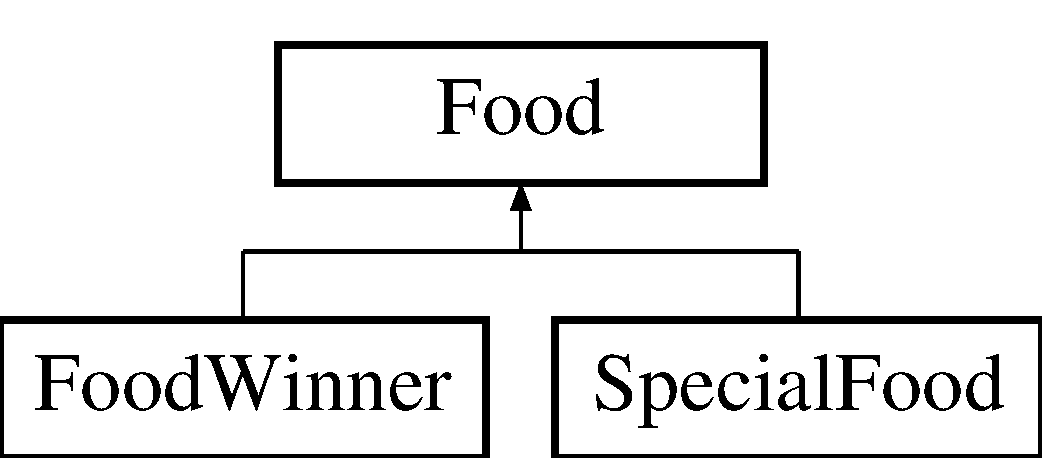
\includegraphics[height=2.000000cm]{classFood}
\end{center}
\end{figure}
\subsection*{\-Public \-Member \-Functions}
\begin{DoxyCompactItemize}
\item 
\hypertarget{classFood_a75d4d7f76fd495cc8133302ca9fdc485}{\hyperlink{classFood_a75d4d7f76fd495cc8133302ca9fdc485}{\-Food} ()}\label{classFood_a75d4d7f76fd495cc8133302ca9fdc485}

\begin{DoxyCompactList}\small\item\em \-Class \-Constructor -\/ loads first image, moves to random location. \-Precondition\-: \-A new instance of game was created. \-Postcondition\-: \-A new piece of food is created with default image. \end{DoxyCompactList}\item 
\hypertarget{classFood_a6f25dffd1fb347c982a53b9a384c611a}{\hyperlink{classFood_a6f25dffd1fb347c982a53b9a384c611a}{$\sim$\-Food} ()}\label{classFood_a6f25dffd1fb347c982a53b9a384c611a}

\begin{DoxyCompactList}\small\item\em \-Class \-Destructor -\/ \-Does \-Nothing. \end{DoxyCompactList}\item 
void \hyperlink{classFood_ad902c4b35177dc47f4f5845cea946b47}{move\-Food} (\hyperlink{classFood}{\-Food} $\ast$other\-Food)
\begin{DoxyCompactList}\small\item\em \-Draws \hyperlink{classFood}{\-Food} in a random location. \-Precondition\-: \-The \hyperlink{classSnake}{\-Snake} head collided with a piece of \hyperlink{classFood}{\-Food} or \hyperlink{classFood}{\-Food} cheat code key was pressed. \-Postcondition\-: \hyperlink{classFood}{\-Food} is moved to a random location on the screen which is not on top of other\-Food. \end{DoxyCompactList}\item 
void \hyperlink{classFood_abb8f6f4e6de3a9c30d821a570227b0b3}{move\-Food} (\hyperlink{classFood}{\-Food} $\ast$other\-Food, int which\-Food)
\begin{DoxyCompactList}\small\item\em \-Draws \hyperlink{classFood}{\-Food} in a random location. \-Precondition\-: \-The \hyperlink{classSnake}{\-Snake} head collided with a piece of \hyperlink{classFood}{\-Food} or \hyperlink{classFood}{\-Food} cheat code key was pressed. \-Postcondition\-: \hyperlink{classFood}{\-Food} is moved to a random location on the screen which is not on top of other\-Food. \end{DoxyCompactList}\item 
void \hyperlink{classFood_a3eb6229d350b6d6dec7256f633c0e603}{move\-Food} (int which\-Food)
\begin{DoxyCompactList}\small\item\em \-Draws \hyperlink{classFood}{\-Food} in a random location. \-Precondition\-: \-The \hyperlink{classSnake}{\-Snake} head collided with a piece of \hyperlink{classFood}{\-Food} or \hyperlink{classFood}{\-Food} cheat code key was pressed. \-Postcondition\-: \hyperlink{classFood}{\-Food} is moved to a random location on the screen which is not on top of other\-Food. \end{DoxyCompactList}\item 
\hypertarget{classFood_a7a286e4848f36fd65ba15d83cf09712d}{void \hyperlink{classFood_a7a286e4848f36fd65ba15d83cf09712d}{pick\-Location} ()}\label{classFood_a7a286e4848f36fd65ba15d83cf09712d}

\begin{DoxyCompactList}\small\item\em \-Picks a random location to move \hyperlink{classFood}{\-Food} to, but does not move \hyperlink{classFood}{\-Food}. \-Precondition\-: \hyperlink{classFood}{\-Food} needs to be moved to a new location. \-Postcondition\-: \-New location is picked for \hyperlink{classFood}{\-Food} to move to. \end{DoxyCompactList}\item 
\-Q\-Rect \hyperlink{classFood_a086048638fd5c0da29fa69594dc1a703}{get\-Rect} ()
\begin{DoxyCompactList}\small\item\em \-Returns rect of \hyperlink{classFood}{\-Food}. \-Precondition\-: \-Any collision detection or paint event that involes the \hyperlink{classFood}{\-Food} occured. \-Postcondition\-: \-The \-Qrect of the \hyperlink{classFood}{\-Food} is returned. \end{DoxyCompactList}\item 
\-Q\-Image \& \hyperlink{classFood_a8c6c5967ba2f578e35b2938381a1efd6}{get\-Image} ()
\begin{DoxyCompactList}\small\item\em \-Returns image of \hyperlink{classFood}{\-Food}. \-Precondition\-: \-Instance of \hyperlink{classGame}{\-Game} called a paint event and the game is started. \-Postcondition\-: \-The image of the \hyperlink{classFood}{\-Food} will be painted on the screen. \end{DoxyCompactList}\end{DoxyCompactItemize}
\subsection*{\-Protected \-Attributes}
\begin{DoxyCompactItemize}
\item 
\hypertarget{classFood_a6cb4da80ded62e777162ed689afff2ec}{int \hyperlink{classFood_a6cb4da80ded62e777162ed689afff2ec}{x}}\label{classFood_a6cb4da80ded62e777162ed689afff2ec}

\begin{DoxyCompactList}\small\item\em \-The x position of \hyperlink{classFood}{\-Food}. \end{DoxyCompactList}\item 
\hypertarget{classFood_aad0125787e9b00210d2a0b0dc94b39c4}{int \hyperlink{classFood_aad0125787e9b00210d2a0b0dc94b39c4}{y}}\label{classFood_aad0125787e9b00210d2a0b0dc94b39c4}

\begin{DoxyCompactList}\small\item\em \-The y position of \hyperlink{classFood}{\-Food}. \end{DoxyCompactList}\item 
\hypertarget{classFood_a53968c7ffd02f4a65201438857efe9bf}{\-Q\-Image \hyperlink{classFood_a53968c7ffd02f4a65201438857efe9bf}{image}}\label{classFood_a53968c7ffd02f4a65201438857efe9bf}

\begin{DoxyCompactList}\small\item\em \-The \-Q\-Image of \hyperlink{classFood}{\-Food}. \end{DoxyCompactList}\item 
\hypertarget{classFood_a1cb41fead62d37b800db81ed9e1f3939}{\-Q\-Rect \hyperlink{classFood_a1cb41fead62d37b800db81ed9e1f3939}{rect}}\label{classFood_a1cb41fead62d37b800db81ed9e1f3939}

\begin{DoxyCompactList}\small\item\em \-The \-Q\-Rect of \hyperlink{classFood}{\-Food}. \end{DoxyCompactList}\end{DoxyCompactItemize}


\subsection{\-Detailed \-Description}
\-A \hyperlink{classFood}{\-Food} piece \-The parent of all food pieces. \-If not inherited, \hyperlink{classFood}{\-Food} represents a red or green \-Apple \-Logo. 

\subsection{\-Member \-Function \-Documentation}
\hypertarget{classFood_a8c6c5967ba2f578e35b2938381a1efd6}{\index{\-Food@{\-Food}!get\-Image@{get\-Image}}
\index{get\-Image@{get\-Image}!Food@{\-Food}}
\subsubsection[{get\-Image}]{\setlength{\rightskip}{0pt plus 5cm}\-Q\-Image \& {\bf \-Food\-::get\-Image} (
\begin{DoxyParamCaption}
{}
\end{DoxyParamCaption}
)}}\label{classFood_a8c6c5967ba2f578e35b2938381a1efd6}


\-Returns image of \hyperlink{classFood}{\-Food}. \-Precondition\-: \-Instance of \hyperlink{classGame}{\-Game} called a paint event and the game is started. \-Postcondition\-: \-The image of the \hyperlink{classFood}{\-Food} will be painted on the screen. 

\begin{DoxyReturn}{\-Returns}
\-Image of \hyperlink{classFood}{\-Food}. 
\end{DoxyReturn}
\hypertarget{classFood_a086048638fd5c0da29fa69594dc1a703}{\index{\-Food@{\-Food}!get\-Rect@{get\-Rect}}
\index{get\-Rect@{get\-Rect}!Food@{\-Food}}
\subsubsection[{get\-Rect}]{\setlength{\rightskip}{0pt plus 5cm}\-Q\-Rect {\bf \-Food\-::get\-Rect} (
\begin{DoxyParamCaption}
{}
\end{DoxyParamCaption}
)}}\label{classFood_a086048638fd5c0da29fa69594dc1a703}


\-Returns rect of \hyperlink{classFood}{\-Food}. \-Precondition\-: \-Any collision detection or paint event that involes the \hyperlink{classFood}{\-Food} occured. \-Postcondition\-: \-The \-Qrect of the \hyperlink{classFood}{\-Food} is returned. 

\begin{DoxyReturn}{\-Returns}
\-The rect of \hyperlink{classFood}{\-Food}. 
\end{DoxyReturn}
\hypertarget{classFood_ad902c4b35177dc47f4f5845cea946b47}{\index{\-Food@{\-Food}!move\-Food@{move\-Food}}
\index{move\-Food@{move\-Food}!Food@{\-Food}}
\subsubsection[{move\-Food}]{\setlength{\rightskip}{0pt plus 5cm}void {\bf \-Food\-::move\-Food} (
\begin{DoxyParamCaption}
\item[{{\bf \-Food} $\ast$}]{other\-Food}
\end{DoxyParamCaption}
)}}\label{classFood_ad902c4b35177dc47f4f5845cea946b47}


\-Draws \hyperlink{classFood}{\-Food} in a random location. \-Precondition\-: \-The \hyperlink{classSnake}{\-Snake} head collided with a piece of \hyperlink{classFood}{\-Food} or \hyperlink{classFood}{\-Food} cheat code key was pressed. \-Postcondition\-: \hyperlink{classFood}{\-Food} is moved to a random location on the screen which is not on top of other\-Food. 


\begin{DoxyParams}{\-Parameters}
{\em $\ast$other\-Food} & \-The other piece of \hyperlink{classFood}{\-Food} on the screen\\
\hline
{\em $\ast$other\-Food} & \-The other piece of \hyperlink{classFood}{\-Food} on the screen. \\
\hline
\end{DoxyParams}
\hypertarget{classFood_abb8f6f4e6de3a9c30d821a570227b0b3}{\index{\-Food@{\-Food}!move\-Food@{move\-Food}}
\index{move\-Food@{move\-Food}!Food@{\-Food}}
\subsubsection[{move\-Food}]{\setlength{\rightskip}{0pt plus 5cm}void {\bf \-Food\-::move\-Food} (
\begin{DoxyParamCaption}
\item[{{\bf \-Food} $\ast$}]{other\-Food, }
\item[{int}]{which\-Food}
\end{DoxyParamCaption}
)}}\label{classFood_abb8f6f4e6de3a9c30d821a570227b0b3}


\-Draws \hyperlink{classFood}{\-Food} in a random location. \-Precondition\-: \-The \hyperlink{classSnake}{\-Snake} head collided with a piece of \hyperlink{classFood}{\-Food} or \hyperlink{classFood}{\-Food} cheat code key was pressed. \-Postcondition\-: \hyperlink{classFood}{\-Food} is moved to a random location on the screen which is not on top of other\-Food. 


\begin{DoxyParams}{\-Parameters}
{\em $\ast$other\-Food} & \-The other piece of \hyperlink{classFood}{\-Food} on the screen. \\
\hline
{\em which\-Food} & \-The integer switch between \hyperlink{classFood}{\-Food} images. \\
\hline
\end{DoxyParams}
\hypertarget{classFood_a3eb6229d350b6d6dec7256f633c0e603}{\index{\-Food@{\-Food}!move\-Food@{move\-Food}}
\index{move\-Food@{move\-Food}!Food@{\-Food}}
\subsubsection[{move\-Food}]{\setlength{\rightskip}{0pt plus 5cm}void {\bf \-Food\-::move\-Food} (
\begin{DoxyParamCaption}
\item[{int}]{which\-Food}
\end{DoxyParamCaption}
)}}\label{classFood_a3eb6229d350b6d6dec7256f633c0e603}


\-Draws \hyperlink{classFood}{\-Food} in a random location. \-Precondition\-: \-The \hyperlink{classSnake}{\-Snake} head collided with a piece of \hyperlink{classFood}{\-Food} or \hyperlink{classFood}{\-Food} cheat code key was pressed. \-Postcondition\-: \hyperlink{classFood}{\-Food} is moved to a random location on the screen which is not on top of other\-Food. 


\begin{DoxyParams}{\-Parameters}
{\em which\-Food} & \-The integer switch between \hyperlink{classFood}{\-Food} images. \\
\hline
\end{DoxyParams}


\-The documentation for this class was generated from the following files\-:\begin{DoxyCompactItemize}
\item 
\hyperlink{Food_8h}{\-Food.\-h}\item 
\hyperlink{Food_8cpp}{\-Food.\-cpp}\end{DoxyCompactItemize}

\hypertarget{classFoodWinner}{\section{\-Food\-Winner \-Class \-Reference}
\label{classFoodWinner}\index{\-Food\-Winner@{\-Food\-Winner}}
}


\-A \hyperlink{classFoodWinner}{\-Food\-Winner} piece \-A daughter of the \hyperlink{classFood}{\-Food} class. \-Represents a \-Linux \-Logo. \-If \hyperlink{classSnake}{\-Snake} collides with \hyperlink{classFoodWinner}{\-Food\-Winner}, a victory screen will occur.  




{\ttfamily \#include $<$\-Food\-Winner.\-h$>$}

\-Inheritance diagram for \-Food\-Winner\-:\begin{figure}[H]
\begin{center}
\leavevmode
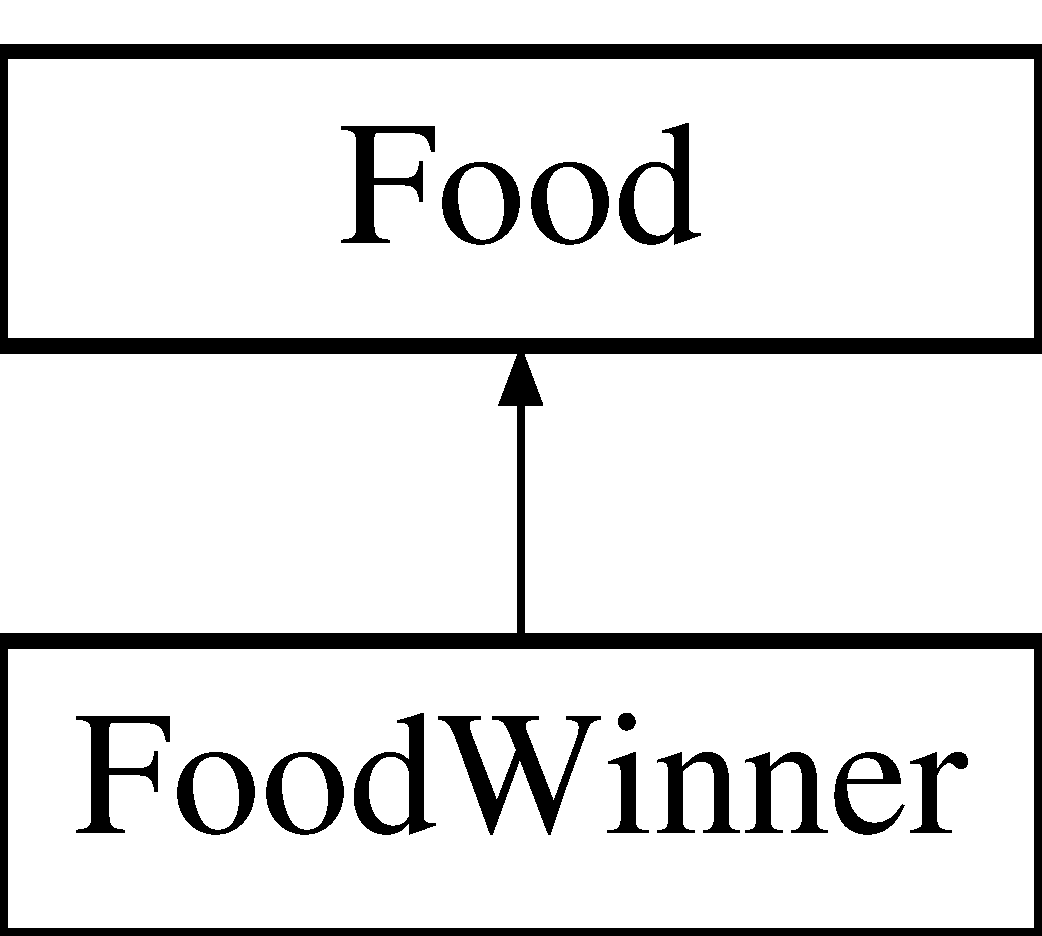
\includegraphics[height=2.000000cm]{classFoodWinner}
\end{center}
\end{figure}
\subsection*{\-Public \-Member \-Functions}
\begin{DoxyCompactItemize}
\item 
\hyperlink{classFoodWinner_a7a2f3f0cefcb12b4ec423f8511aefd01}{\-Food\-Winner} ()
\item 
\hyperlink{classFoodWinner_aea338ffe14d81d42a6298ebeab930621}{$\sim$\-Food\-Winner} ()
\end{DoxyCompactItemize}


\subsection{\-Detailed \-Description}
\-A \hyperlink{classFoodWinner}{\-Food\-Winner} piece \-A daughter of the \hyperlink{classFood}{\-Food} class. \-Represents a \-Linux \-Logo. \-If \hyperlink{classSnake}{\-Snake} collides with \hyperlink{classFoodWinner}{\-Food\-Winner}, a victory screen will occur. 

\subsection{\-Constructor \& \-Destructor \-Documentation}
\hypertarget{classFoodWinner_a7a2f3f0cefcb12b4ec423f8511aefd01}{\index{\-Food\-Winner@{\-Food\-Winner}!\-Food\-Winner@{\-Food\-Winner}}
\index{\-Food\-Winner@{\-Food\-Winner}!FoodWinner@{\-Food\-Winner}}
\subsubsection[{\-Food\-Winner}]{\setlength{\rightskip}{0pt plus 5cm}{\bf \-Food\-Winner\-::\-Food\-Winner} (
\begin{DoxyParamCaption}
{}
\end{DoxyParamCaption}
)}}\label{classFoodWinner_a7a2f3f0cefcb12b4ec423f8511aefd01}
\-Class \-Constructor -\/ loads first image, moves to random location. \-Precondition\-: \-A new instance of game was created. \-Postcondition\-: \-A new piece of food is created with \-Linux logo image. \hypertarget{classFoodWinner_aea338ffe14d81d42a6298ebeab930621}{\index{\-Food\-Winner@{\-Food\-Winner}!$\sim$\-Food\-Winner@{$\sim$\-Food\-Winner}}
\index{$\sim$\-Food\-Winner@{$\sim$\-Food\-Winner}!FoodWinner@{\-Food\-Winner}}
\subsubsection[{$\sim$\-Food\-Winner}]{\setlength{\rightskip}{0pt plus 5cm}{\bf \-Food\-Winner\-::$\sim$\-Food\-Winner} (
\begin{DoxyParamCaption}
{}
\end{DoxyParamCaption}
)}}\label{classFoodWinner_aea338ffe14d81d42a6298ebeab930621}
\-Class \-Destructor -\/ \-Does \-Nothing 

\-The documentation for this class was generated from the following files\-:\begin{DoxyCompactItemize}
\item 
\hyperlink{FoodWinner_8h}{\-Food\-Winner.\-h}\item 
\hyperlink{FoodWinner_8cpp}{\-Food\-Winner.\-cpp}\end{DoxyCompactItemize}

\hypertarget{classGame}{\section{\-Game \-Class \-Reference}
\label{classGame}\index{\-Game@{\-Game}}
}


\-The \hyperlink{classSnake}{\-Snake} \hyperlink{classGame}{\-Game} \-Logic. \-This class contains the logic that makes up the \hyperlink{classSnake}{\-Snake} \hyperlink{classGame}{\-Game}.  




{\ttfamily \#include $<$\-Game.\-h$>$}

\subsection*{\-Public \-Member \-Functions}
\begin{DoxyCompactItemize}
\item 
\hypertarget{classGame_ae3c64a8dd73de0a99849db8ec0e9a86c}{\hyperlink{classGame_ae3c64a8dd73de0a99849db8ec0e9a86c}{\-Game} (\-Q\-Widget $\ast$parent=0)}\label{classGame_ae3c64a8dd73de0a99849db8ec0e9a86c}

\begin{DoxyCompactList}\small\item\em \-Class \-Constructor -\/ initializes the data members to default values and creates dynamically allocated memory. \-Precondition\-: \hyperlink{classGame}{\-Game} object has been created. \-Postcondition\-: \-Intro screen 1 is displayed. \end{DoxyCompactList}\item 
\hypertarget{classGame_ae3d112ca6e0e55150d2fdbc704474530}{\hyperlink{classGame_ae3d112ca6e0e55150d2fdbc704474530}{$\sim$\-Game} ()}\label{classGame_ae3d112ca6e0e55150d2fdbc704474530}

\begin{DoxyCompactList}\small\item\em \-Class \-Destructor -\/ \-Deletes dynamically allocated objects (special\-Food, food\-Winner, food, and snake). \end{DoxyCompactList}\end{DoxyCompactItemize}
\subsection*{\-Protected \-Member \-Functions}
\begin{DoxyCompactItemize}
\item 
void \hyperlink{classGame_a5c408cb3451b941a5d86757096086f95}{paint\-Event} (\-Q\-Paint\-Event $\ast$event)
\begin{DoxyCompactList}\small\item\em \-Paints the necessary object on the screen. \-Precondition\-: a \-Q\-Paint\-Event is called. \-Postcondition\-: \-Necessary objects are painted on the screen. \end{DoxyCompactList}\item 
void \hyperlink{classGame_a6a870e7567a5d57e4060d8140644a01b}{timer\-Event} (\-Q\-Timer\-Event $\ast$event)
\begin{DoxyCompactList}\small\item\em \-Occurs when ever a timer event is called. \-Precondition\-: a \-Q\-Timer\-Event is called. \-Postcondition\-: \-If game is started and the direction has not changed, then the \hyperlink{classSnake}{\-Snake} is moved and collsion detection is run (check\-Collision is called). \-Next, changed\-Dir is set to false and \-Q\-Paint\-Event (repaint) is called. \end{DoxyCompactList}\item 
void \hyperlink{classGame_a08d72c91a6daedc8fa48194253f5e567}{key\-Press\-Event} (\-Q\-Key\-Event $\ast$event)
\begin{DoxyCompactList}\small\item\em \-Carries out the required actions for the specific key. \-Precondition\-: a \-Q\-Key\-Event is called. (a key is pressed) \-Postcondition\-: \-Actions for specified key are carried out. \end{DoxyCompactList}\item 
\hypertarget{classGame_ae8638ccdb0ef3bf39a6affa30aa1258f}{void \hyperlink{classGame_ae8638ccdb0ef3bf39a6affa30aa1258f}{start\-Game} ()}\label{classGame_ae8638ccdb0ef3bf39a6affa30aa1258f}

\begin{DoxyCompactList}\small\item\em \-If game is not started, resets data members to default values, deletes \hyperlink{classSnake}{\-Snake}, creates a new \hyperlink{classSnake}{\-Snake} to default length and position, and moves food. \-Precondition\-: \hyperlink{classGame}{\-Game} is not started and a '\-Y' or '\-N' was pressed during intro \-Screen 2. \-Postcondition\-: \hyperlink{classGame}{\-Game} is started and \hyperlink{classSnake}{\-Snake} is centered on screen. \end{DoxyCompactList}\item 
\hypertarget{classGame_a9d9a79a0f7df3c7e55a3103c04ecbc87}{void \hyperlink{classGame_a9d9a79a0f7df3c7e55a3103c04ecbc87}{pause\-Game} ()}\label{classGame_a9d9a79a0f7df3c7e55a3103c04ecbc87}

\begin{DoxyCompactList}\small\item\em \-Pauses and \-Unpauses a started game. \-Precondition\-: \hyperlink{classGame}{\-Game} is started and '\-P' is pressed, or \hyperlink{classGame}{\-Game} is paused and '\-P' or a directional key is pressed. \-Postcondition\-: \-If game is started, the game is paused. \-If game is paused, game is unpaused. \end{DoxyCompactList}\item 
\hypertarget{classGame_a9ec1a0c5ee8b5e06fa429162b5e73564}{void \hyperlink{classGame_a9ec1a0c5ee8b5e06fa429162b5e73564}{stop\-Game} ()}\label{classGame_a9ec1a0c5ee8b5e06fa429162b5e73564}

\begin{DoxyCompactList}\small\item\em \-Stops the game and the timer, sets up variables to paint the game\-Over\-Screen, and calls a paint event. \-Precondition\-: \hyperlink{classSnake}{\-Snake} makes an illegal collision or any key is pressed during the \-Blue \-Screen of \-Death. \-Postcondition\-: \-The paint event will display the game\-Over\-Screen. \end{DoxyCompactList}\item 
\hypertarget{classGame_a6a02e00bf61930576156c6c59b817a25}{void \hyperlink{classGame_a6a02e00bf61930576156c6c59b817a25}{victory} ()}\label{classGame_a6a02e00bf61930576156c6c59b817a25}

\begin{DoxyCompactList}\small\item\em \-Stops the game and the timer, sets up variables to paint the victory\-Screen, and calls a paint event. \-Precondition\-: \-If snake collides with food\-Winner, game is started and '\-V' is pressed, or grow\-Count == 315. \-Postcondition\-: \-The paint event will display the victory\-Screen. \end{DoxyCompactList}\item 
\hypertarget{classGame_a21cdf5a4c8decb922bbb17ae6e55f636}{void \hyperlink{classGame_a21cdf5a4c8decb922bbb17ae6e55f636}{blue\-Screen\-Death} ()}\label{classGame_a21cdf5a4c8decb922bbb17ae6e55f636}

\begin{DoxyCompactList}\small\item\em \-Stops the timer, sets up variables to paint the \-Blue \-Screen of \-Death, sets points to zero, and calls a paint event. \-Precondition\-: \-If snake collides with special\-Food, or game is started and '8' is pressed. \-Postcondition\-: \-Points are set to zero and the paint event will display the \-Blue \-Screen of \-Death. \end{DoxyCompactList}\item 
void \hyperlink{classGame_a878615d81c26a1c5b62992f741f63e6d}{game\-Over\-Screen} (\-Q\-Painter \&painter)
\begin{DoxyCompactList}\small\item\em \-The screen that is displayed when a \hyperlink{classGame}{\-Game} \-Over occurs. \-Precondition\-: \-Paint event is called and game\-Over is true. \-Postcondition\-: game\-Over\-Screen is displayed. \end{DoxyCompactList}\item 
void \hyperlink{classGame_acdc0eaef5b29ea5d73edf8c908cf8dc7}{victory\-Screen} (\-Q\-Painter \&painter)
\begin{DoxyCompactList}\small\item\em \-The screen that is displayed when a \-Victory occurs. \-Precondition\-: \-Paint event is called and game\-Won is true. \-Postcondition\-: victory\-Screen is displayed. \end{DoxyCompactList}\item 
void \hyperlink{classGame_ad8ec719e40e94a3a1a059fd2f25b5dd1}{get\-Points} (\-Q\-Painter \&painter)
\begin{DoxyCompactList}\small\item\em \-Paints points on the status bar on the iphone. \-Precondition\-: \-Paint event is called and either game\-Started or \-B\-S\-O\-D is true. \-Postcondition\-: \-Points are displayed on status bar of iphone. \end{DoxyCompactList}\item 
void \hyperlink{classGame_a34e40db4bb49df422db3b120de17e5b6}{intro\-Screen} (\-Q\-Painter \&painter)
\begin{DoxyCompactList}\small\item\em \-Paints the intro screens on the screen of the iphone. \-Precondition\-: \-Paint event is called and either intro\-Prompt1 or intro\-Prompt2 is true. \-Postcondition\-: \-Either intro screen 1 or intro screen 2 is displayed. \end{DoxyCompactList}\item 
\hypertarget{classGame_a71802e92f514d4b79f3168b70d7217a6}{void \hyperlink{classGame_a71802e92f514d4b79f3168b70d7217a6}{check\-Collision} ()}\label{classGame_a71802e92f514d4b79f3168b70d7217a6}

\begin{DoxyCompactList}\small\item\em \-Carries out actions if snake collided with something. \-Precondition\-: \-The \hyperlink{classSnake}{\-Snake} is moved by a directional key press or a timer event. \-Postcondition\-: \-Specific action carried out according to what the snake collided with. \end{DoxyCompactList}\end{DoxyCompactItemize}
\subsection*{\-Private \-Attributes}
\begin{DoxyCompactItemize}
\item 
\hypertarget{classGame_ac6002315e7c8ba1da4fe7a763fe442b2}{\hyperlink{classSnake}{\-Snake} $\ast$ \hyperlink{classGame_ac6002315e7c8ba1da4fe7a763fe442b2}{snake}}\label{classGame_ac6002315e7c8ba1da4fe7a763fe442b2}

\begin{DoxyCompactList}\small\item\em \-The infinitely growing snake. \end{DoxyCompactList}\item 
\hypertarget{classGame_a9af4c00a595db1e8a377189fbfdfdbcd}{\hyperlink{classFood}{\-Food} $\ast$ \hyperlink{classGame_a9af4c00a595db1e8a377189fbfdfdbcd}{food}}\label{classGame_a9af4c00a595db1e8a377189fbfdfdbcd}

\begin{DoxyCompactList}\small\item\em \-The normal piece of \hyperlink{classFood}{\-Food}, red or green apple logo. \-If the \hyperlink{classSnake}{\-Snake} eats this \hyperlink{classFood}{\-Food}, the \hyperlink{classSnake}{\-Snake} will grow one \hyperlink{classSnakeBlock}{\-Snake\-Block}. \end{DoxyCompactList}\item 
\hypertarget{classGame_aad79a1e2a336f39acefdc46bd091110b}{\hyperlink{classSpecialFood}{\-Special\-Food} $\ast$ \hyperlink{classGame_aad79a1e2a336f39acefdc46bd091110b}{special\-Food}}\label{classGame_aad79a1e2a336f39acefdc46bd091110b}

\begin{DoxyCompactList}\small\item\em \-The special piece of \hyperlink{classFood}{\-Food}, \-The \-Windows 8 logo. \-If the \hyperlink{classSnake}{\-Snake} eats this \hyperlink{classFood}{\-Food}, the game will go into a \-Blue \-Screen of \-Death \hyperlink{classGame}{\-Game} over in which the user loses all points. \-This will spawn every ten grows for 100 paint events. \end{DoxyCompactList}\item 
\hypertarget{classGame_ad5fae274ed08a2f7e2e940f28c4dcafe}{\hyperlink{classFoodWinner}{\-Food\-Winner} $\ast$ \hyperlink{classGame_ad5fae274ed08a2f7e2e940f28c4dcafe}{food\-Winner}}\label{classGame_ad5fae274ed08a2f7e2e940f28c4dcafe}

\begin{DoxyCompactList}\small\item\em \-The winning piece of \hyperlink{classFood}{\-Food}, \-The \-Linux logo. \-If the \hyperlink{classSnake}{\-Snake} eats this \hyperlink{classFood}{\-Food}, the game will go into a \-Victory \-Screen in which the game ends and a special screen is displayed. \-This will spawn after the special\-Food has been painted 100 times. \-It will be painted for 100 paint events, and then disappear. \end{DoxyCompactList}\item 
\hypertarget{classGame_a096ce28dfd515112ffac0a6b25a7b969}{\hyperlink{classIphone}{\-Iphone} \hyperlink{classGame_a096ce28dfd515112ffac0a6b25a7b969}{iphone}}\label{classGame_a096ce28dfd515112ffac0a6b25a7b969}

\begin{DoxyCompactList}\small\item\em \-The \hyperlink{classIphone}{\-Iphone} border around the game. \end{DoxyCompactList}\item 
\hypertarget{classGame_aceecf6c9057f65306e5086644d3a621f}{int \hyperlink{classGame_aceecf6c9057f65306e5086644d3a621f}{timer\-Id}}\label{classGame_aceecf6c9057f65306e5086644d3a621f}

\begin{DoxyCompactList}\small\item\em \-The unique timer identifier that is returned from start\-Timer(). \-It is passed to kill\-Timer(int id) in order to stop the timer. \end{DoxyCompactList}\item 
\hypertarget{classGame_aba9da13645292bf746be23ea698c1919}{int \hyperlink{classGame_aba9da13645292bf746be23ea698c1919}{speed\-Delay}}\label{classGame_aba9da13645292bf746be23ea698c1919}

\begin{DoxyCompactList}\small\item\em \-The timer delay that controls the speed. \-It is passed to start\-Timer() in order to start the timer. \end{DoxyCompactList}\item 
\hypertarget{classGame_acf48e7c6cc26020e3cb205a0aebd63bd}{unsigned int \hyperlink{classGame_acf48e7c6cc26020e3cb205a0aebd63bd}{points}}\label{classGame_acf48e7c6cc26020e3cb205a0aebd63bd}

\begin{DoxyCompactList}\small\item\em \-The number of points the user has accumulated. \end{DoxyCompactList}\item 
\hypertarget{classGame_a937bcfe7d65bcec1849b70a1ed0f9b30}{unsigned int \hyperlink{classGame_a937bcfe7d65bcec1849b70a1ed0f9b30}{point\-Multi}}\label{classGame_a937bcfe7d65bcec1849b70a1ed0f9b30}

\begin{DoxyCompactList}\small\item\em \-The points multiplier, this variable will be multiplied with the points that the user earns during each grow. \-The \-User sets this variable during 1st intro screens. \end{DoxyCompactList}\item 
\hypertarget{classGame_af942acedb59e3d6a9a57565f28aa312d}{bool \hyperlink{classGame_af942acedb59e3d6a9a57565f28aa312d}{wrap\-Around}}\label{classGame_af942acedb59e3d6a9a57565f28aa312d}

\begin{DoxyCompactList}\small\item\em \-This control what logic is used when the \hyperlink{classSnake}{\-Snake} hits the wall. \-The \-User sets this variable during 2nd intro screens. \-If \-False, a game over will occur when the \hyperlink{classSnake}{\-Snake} hits the wall. \-If \-True, the \hyperlink{classSnake}{\-Snake} will wrap around to the other side of the screen when it hits the wall. \end{DoxyCompactList}\item 
\hypertarget{classGame_a5dc3b4a5881de404704396843f240407}{bool \hyperlink{classGame_a5dc3b4a5881de404704396843f240407}{intro\-Prompt1}}\label{classGame_a5dc3b4a5881de404704396843f240407}

\begin{DoxyCompactList}\small\item\em \-Controls when intro prompt 1 is displayed, and what actions to take, when intro prompt 1, is displayed during a key press event. \end{DoxyCompactList}\item 
\hypertarget{classGame_aff3156d47d93ce108ee1d25da3ceea3c}{bool \hyperlink{classGame_aff3156d47d93ce108ee1d25da3ceea3c}{intro\-Prompt2}}\label{classGame_aff3156d47d93ce108ee1d25da3ceea3c}

\begin{DoxyCompactList}\small\item\em \-Controls when intro prompt 2 is displayed, and what actions to take, when intro prompt 2 is displayed, during a key press event. \end{DoxyCompactList}\item 
\hypertarget{classGame_af3d6a9c87d9278503529d5b62dba4077}{bool \hyperlink{classGame_af3d6a9c87d9278503529d5b62dba4077}{game\-Started}}\label{classGame_af3d6a9c87d9278503529d5b62dba4077}

\begin{DoxyCompactList}\small\item\em \-Whether or not the game is started. \-True when game is started, otherwise \-False. \end{DoxyCompactList}\item 
\hypertarget{classGame_a21f9857b2d4b38b97ec90b9c2ce3413d}{bool \hyperlink{classGame_a21f9857b2d4b38b97ec90b9c2ce3413d}{game\-Over}}\label{classGame_a21f9857b2d4b38b97ec90b9c2ce3413d}

\begin{DoxyCompactList}\small\item\em \-Whether or not a game over has occured. \-True when a game over has occur, otherwise \-False. \-Controls when \hyperlink{classGame}{\-Game} \-Over \-Screen is displayed. \end{DoxyCompactList}\item 
\hypertarget{classGame_a55d6d8def7c867d94f8ae820884f1aff}{bool \hyperlink{classGame_a55d6d8def7c867d94f8ae820884f1aff}{game\-Won}}\label{classGame_a55d6d8def7c867d94f8ae820884f1aff}

\begin{DoxyCompactList}\small\item\em \-Whether or not a victory (the game has been won) has occured. \-True when a victory has occured, otherwise \-False. \-Controls when \-Victory \-Screen is displayed. \end{DoxyCompactList}\item 
\hypertarget{classGame_a2988aab32f3a086595ba3d1d675d9bee}{bool \hyperlink{classGame_a2988aab32f3a086595ba3d1d675d9bee}{game\-Ended}}\label{classGame_a2988aab32f3a086595ba3d1d675d9bee}

\begin{DoxyCompactList}\small\item\em \-Whether or not a victory or a game over has occured. \-True when a victory or a game over has occured, otherwise \-False. \-Controls what actions to take during a key press event, when a victory or a game over has occured. \end{DoxyCompactList}\item 
\hypertarget{classGame_aea8eb9e9304b43e6ecc2c4a0377d3155}{bool \hyperlink{classGame_aea8eb9e9304b43e6ecc2c4a0377d3155}{b\-S\-O\-D}}\label{classGame_aea8eb9e9304b43e6ecc2c4a0377d3155}

\begin{DoxyCompactList}\small\item\em \-Whether or not a \-Blue screen of death has occured. \-True when a \-Blue screen of death has occured, otherwise \-False. \-Controls when \-Blue screen of death is displayed, and what actions to take, when \-Blue screen of death is displayed, during a key press event. \end{DoxyCompactList}\item 
\hypertarget{classGame_a255049de8fb46a9f00946631e3121c03}{bool \hyperlink{classGame_a255049de8fb46a9f00946631e3121c03}{paused}}\label{classGame_a255049de8fb46a9f00946631e3121c03}

\begin{DoxyCompactList}\small\item\em \-Whether or not the game is paused. \-True when the game is paused, otherwise \-False. \end{DoxyCompactList}\item 
\hypertarget{classGame_a505ba53ef639736e8a4edb222de00f82}{bool \hyperlink{classGame_a505ba53ef639736e8a4edb222de00f82}{changed\-Dir}}\label{classGame_a505ba53ef639736e8a4edb222de00f82}

\begin{DoxyCompactList}\small\item\em \-Whether or not the snake has changed directions before the last tiemr event. \-True when the snake has changed directions before the last timer event, otherwise \-False. \end{DoxyCompactList}\item 
\hypertarget{classGame_af62d7b5c18f6cdd90dd80f98cb783bd9}{char \hyperlink{classGame_af62d7b5c18f6cdd90dd80f98cb783bd9}{last\-Dir}}\label{classGame_af62d7b5c18f6cdd90dd80f98cb783bd9}

\begin{DoxyCompactList}\small\item\em \-Stores the last valid direction of the \hyperlink{classSnake}{\-Snake}. \end{DoxyCompactList}\item 
\hypertarget{classGame_ae2a3b6bed2a17912ba8722958d5e0caa}{unsigned int \hyperlink{classGame_ae2a3b6bed2a17912ba8722958d5e0caa}{grow\-Count}}\label{classGame_ae2a3b6bed2a17912ba8722958d5e0caa}

\begin{DoxyCompactList}\small\item\em \-The number of times the snake has grown. \-Controls when to start displaying special\-Food. \-Once grow\-Count \% 10 == 0, special\-Food is painted. \end{DoxyCompactList}\item 
\hypertarget{classGame_ac0bd70f6892c174d1d7c65150e9c6fb5}{unsigned int \hyperlink{classGame_ac0bd70f6892c174d1d7c65150e9c6fb5}{spawn\-Winner\-Count}}\label{classGame_ac0bd70f6892c174d1d7c65150e9c6fb5}

\begin{DoxyCompactList}\small\item\em \-The number of times the special food has been painted. \-Controls when ro start displaying food\-Winner. \-Once spawn\-Winner\-Count \% 1000 == 0, food\-Winner is painted. \end{DoxyCompactList}\item 
\hypertarget{classGame_a4807181a3e27197af61277273aae86b4}{bool \hyperlink{classGame_a4807181a3e27197af61277273aae86b4}{death\-Spawn}}\label{classGame_a4807181a3e27197af61277273aae86b4}

\begin{DoxyCompactList}\small\item\em \-Whether or not the special\-Food will be painted. \-True when a special\-Food will be painted, otherwise \-False. \-Controls when special\-Food is displayed, and what actions to take, when special\-Food is displayed, during a key press event or during check\-Collision. \end{DoxyCompactList}\item 
\hypertarget{classGame_a5c937032c95deccc527887635cc2ac57}{bool \hyperlink{classGame_a5c937032c95deccc527887635cc2ac57}{win\-Spawn}}\label{classGame_a5c937032c95deccc527887635cc2ac57}

\begin{DoxyCompactList}\small\item\em \-Whether or not the food\-Winner will be painted. \-True when a food\-Winner will be painted, otherwise \-False. \-Controls when food\-Winner is displayed, and what actions to take, when food\-Winner is displayed, during a key press event or during check\-Collision. \end{DoxyCompactList}\item 
\hypertarget{classGame_a2f69ee950ab7ae5ac9df9549aac3458e}{int \hyperlink{classGame_a2f69ee950ab7ae5ac9df9549aac3458e}{death\-Counter}}\label{classGame_a2f69ee950ab7ae5ac9df9549aac3458e}

\begin{DoxyCompactList}\small\item\em \-Increments everytime special\-Food is painted. \-Controls when to stop displaying special\-Food. \-Once death\-Counter \% 100 == 0, special\-Food is no longer painted. \end{DoxyCompactList}\item 
\hypertarget{classGame_ad1b4ed65c72b1b35259c52f0d7246dd5}{int \hyperlink{classGame_ad1b4ed65c72b1b35259c52f0d7246dd5}{win\-Counter}}\label{classGame_ad1b4ed65c72b1b35259c52f0d7246dd5}

\begin{DoxyCompactList}\small\item\em \-Increments everytime food\-Winner is painted. \-Controls when to stop displaying food\-Winner. \-Once win\-Counter \% 100 == 0, food\-Winner is no longer painted. \end{DoxyCompactList}\item 
\hypertarget{classGame_a0b895214583cabcae16d9d1be5a00aab}{bool \hyperlink{classGame_a0b895214583cabcae16d9d1be5a00aab}{do\-One\-Time}}\label{classGame_a0b895214583cabcae16d9d1be5a00aab}

\begin{DoxyCompactList}\small\item\em \-Controls whether or not to move and start displaying food\-Winner or special\-Food. \end{DoxyCompactList}\item 
\hypertarget{classGame_ab4986d9d9139d5438a086b406b4311e4}{bool \hyperlink{classGame_ab4986d9d9139d5438a086b406b4311e4}{fix\-Count}}\label{classGame_ab4986d9d9139d5438a086b406b4311e4}

\begin{DoxyCompactList}\small\item\em \-Controls whether or not to fix the grow count, depending on the spawn of special\-Food. \end{DoxyCompactList}\item 
\hypertarget{classGame_ae5a98023415893d7fb8876e6d6662466}{int \hyperlink{classGame_ae5a98023415893d7fb8876e6d6662466}{switch\-Food}}\label{classGame_ae5a98023415893d7fb8876e6d6662466}

\begin{DoxyCompactList}\small\item\em \-Controls which apple is to be displayed. \-If 0, then green apple is displayed \-If 1, then red apple is displayed. \end{DoxyCompactList}\item 
\hypertarget{classGame_a04465acd56797ce91dd05167a6a094aa}{\-Q\-Image \hyperlink{classGame_a04465acd56797ce91dd05167a6a094aa}{blue\-Screen\-Image}}\label{classGame_a04465acd56797ce91dd05167a6a094aa}

\begin{DoxyCompactList}\small\item\em \-This is the \-Q\-Image of the screen that will be displayed when the \hyperlink{classSnake}{\-Snake} eats a \-Windows 8 logo. \end{DoxyCompactList}\item 
\hypertarget{classGame_a56dc55af7346a05f0c5e63fc334a193b}{\-Q\-Rect \hyperlink{classGame_a56dc55af7346a05f0c5e63fc334a193b}{blue\-Screen\-Rect}}\label{classGame_a56dc55af7346a05f0c5e63fc334a193b}

\begin{DoxyCompactList}\small\item\em \-This is the \-Q\-Rect of the screen that will be displayed when the \hyperlink{classSnake}{\-Snake} eats a \-Windows 8 logo. \end{DoxyCompactList}\item 
\hypertarget{classGame_a64ed5ba3c707a1bc23eeca263d8707f3}{\-Q\-Image \hyperlink{classGame_a64ed5ba3c707a1bc23eeca263d8707f3}{victory\-Screen\-Image}}\label{classGame_a64ed5ba3c707a1bc23eeca263d8707f3}

\begin{DoxyCompactList}\small\item\em \-This is the \-Q\-Image of the screen that will be displayed when the \hyperlink{classSnake}{\-Snake} eats a \-Linux logo. \end{DoxyCompactList}\item 
\hypertarget{classGame_a5917841987549510b5cb274727a8431e}{\-Q\-Rect \hyperlink{classGame_a5917841987549510b5cb274727a8431e}{victory\-Screen\-Rect}}\label{classGame_a5917841987549510b5cb274727a8431e}

\begin{DoxyCompactList}\small\item\em \-This is the \-Q\-Rect of the screen that will be displayed when the \hyperlink{classSnake}{\-Snake} eats a \-Linux logo. \end{DoxyCompactList}\end{DoxyCompactItemize}


\subsection{\-Detailed \-Description}
\-The \hyperlink{classSnake}{\-Snake} \hyperlink{classGame}{\-Game} \-Logic. \-This class contains the logic that makes up the \hyperlink{classSnake}{\-Snake} \hyperlink{classGame}{\-Game}. 

\subsection{\-Member \-Function \-Documentation}
\hypertarget{classGame_a878615d81c26a1c5b62992f741f63e6d}{\index{\-Game@{\-Game}!game\-Over\-Screen@{game\-Over\-Screen}}
\index{game\-Over\-Screen@{game\-Over\-Screen}!Game@{\-Game}}
\subsubsection[{game\-Over\-Screen}]{\setlength{\rightskip}{0pt plus 5cm}void {\bf \-Game\-::game\-Over\-Screen} (
\begin{DoxyParamCaption}
\item[{\-Q\-Painter \&}]{painter}
\end{DoxyParamCaption}
)\hspace{0.3cm}{\ttfamily  \mbox{[}protected\mbox{]}}}}\label{classGame_a878615d81c26a1c5b62992f741f63e6d}


\-The screen that is displayed when a \hyperlink{classGame}{\-Game} \-Over occurs. \-Precondition\-: \-Paint event is called and game\-Over is true. \-Postcondition\-: game\-Over\-Screen is displayed. 


\begin{DoxyParams}{\-Parameters}
{\em \-Q\-T} & \-Qpainter object reference. \\
\hline
\end{DoxyParams}
\hypertarget{classGame_ad8ec719e40e94a3a1a059fd2f25b5dd1}{\index{\-Game@{\-Game}!get\-Points@{get\-Points}}
\index{get\-Points@{get\-Points}!Game@{\-Game}}
\subsubsection[{get\-Points}]{\setlength{\rightskip}{0pt plus 5cm}void {\bf \-Game\-::get\-Points} (
\begin{DoxyParamCaption}
\item[{\-Q\-Painter \&}]{painter}
\end{DoxyParamCaption}
)\hspace{0.3cm}{\ttfamily  \mbox{[}protected\mbox{]}}}}\label{classGame_ad8ec719e40e94a3a1a059fd2f25b5dd1}


\-Paints points on the status bar on the iphone. \-Precondition\-: \-Paint event is called and either game\-Started or \-B\-S\-O\-D is true. \-Postcondition\-: \-Points are displayed on status bar of iphone. 


\begin{DoxyParams}{\-Parameters}
{\em \-Q\-T} & \-Qpainter object reference. \\
\hline
\end{DoxyParams}
\hypertarget{classGame_a34e40db4bb49df422db3b120de17e5b6}{\index{\-Game@{\-Game}!intro\-Screen@{intro\-Screen}}
\index{intro\-Screen@{intro\-Screen}!Game@{\-Game}}
\subsubsection[{intro\-Screen}]{\setlength{\rightskip}{0pt plus 5cm}void {\bf \-Game\-::intro\-Screen} (
\begin{DoxyParamCaption}
\item[{\-Q\-Painter \&}]{painter}
\end{DoxyParamCaption}
)\hspace{0.3cm}{\ttfamily  \mbox{[}protected\mbox{]}}}}\label{classGame_a34e40db4bb49df422db3b120de17e5b6}


\-Paints the intro screens on the screen of the iphone. \-Precondition\-: \-Paint event is called and either intro\-Prompt1 or intro\-Prompt2 is true. \-Postcondition\-: \-Either intro screen 1 or intro screen 2 is displayed. 


\begin{DoxyParams}{\-Parameters}
{\em \-Q\-T} & \-Qpainter object reference. \\
\hline
\end{DoxyParams}
\hypertarget{classGame_a08d72c91a6daedc8fa48194253f5e567}{\index{\-Game@{\-Game}!key\-Press\-Event@{key\-Press\-Event}}
\index{key\-Press\-Event@{key\-Press\-Event}!Game@{\-Game}}
\subsubsection[{key\-Press\-Event}]{\setlength{\rightskip}{0pt plus 5cm}void {\bf \-Game\-::key\-Press\-Event} (
\begin{DoxyParamCaption}
\item[{\-Q\-Key\-Event $\ast$}]{event}
\end{DoxyParamCaption}
)\hspace{0.3cm}{\ttfamily  \mbox{[}protected\mbox{]}}}}\label{classGame_a08d72c91a6daedc8fa48194253f5e567}


\-Carries out the required actions for the specific key. \-Precondition\-: a \-Q\-Key\-Event is called. (a key is pressed) \-Postcondition\-: \-Actions for specified key are carried out. 


\begin{DoxyParams}{\-Parameters}
{\em $\ast$event} & \-Q\-T event pointer \\
\hline
\end{DoxyParams}
\hypertarget{classGame_a5c408cb3451b941a5d86757096086f95}{\index{\-Game@{\-Game}!paint\-Event@{paint\-Event}}
\index{paint\-Event@{paint\-Event}!Game@{\-Game}}
\subsubsection[{paint\-Event}]{\setlength{\rightskip}{0pt plus 5cm}void {\bf \-Game\-::paint\-Event} (
\begin{DoxyParamCaption}
\item[{\-Q\-Paint\-Event $\ast$}]{event}
\end{DoxyParamCaption}
)\hspace{0.3cm}{\ttfamily  \mbox{[}protected\mbox{]}}}}\label{classGame_a5c408cb3451b941a5d86757096086f95}


\-Paints the necessary object on the screen. \-Precondition\-: a \-Q\-Paint\-Event is called. \-Postcondition\-: \-Necessary objects are painted on the screen. 


\begin{DoxyParams}{\-Parameters}
{\em $\ast$event} & \-Q\-T event pointer \\
\hline
\end{DoxyParams}
\hypertarget{classGame_a6a870e7567a5d57e4060d8140644a01b}{\index{\-Game@{\-Game}!timer\-Event@{timer\-Event}}
\index{timer\-Event@{timer\-Event}!Game@{\-Game}}
\subsubsection[{timer\-Event}]{\setlength{\rightskip}{0pt plus 5cm}void {\bf \-Game\-::timer\-Event} (
\begin{DoxyParamCaption}
\item[{\-Q\-Timer\-Event $\ast$}]{event}
\end{DoxyParamCaption}
)\hspace{0.3cm}{\ttfamily  \mbox{[}protected\mbox{]}}}}\label{classGame_a6a870e7567a5d57e4060d8140644a01b}


\-Occurs when ever a timer event is called. \-Precondition\-: a \-Q\-Timer\-Event is called. \-Postcondition\-: \-If game is started and the direction has not changed, then the \hyperlink{classSnake}{\-Snake} is moved and collsion detection is run (check\-Collision is called). \-Next, changed\-Dir is set to false and \-Q\-Paint\-Event (repaint) is called. 


\begin{DoxyParams}{\-Parameters}
{\em $\ast$event} & \-Q\-T event pointer \\
\hline
\end{DoxyParams}
\hypertarget{classGame_acdc0eaef5b29ea5d73edf8c908cf8dc7}{\index{\-Game@{\-Game}!victory\-Screen@{victory\-Screen}}
\index{victory\-Screen@{victory\-Screen}!Game@{\-Game}}
\subsubsection[{victory\-Screen}]{\setlength{\rightskip}{0pt plus 5cm}void {\bf \-Game\-::victory\-Screen} (
\begin{DoxyParamCaption}
\item[{\-Q\-Painter \&}]{painter}
\end{DoxyParamCaption}
)\hspace{0.3cm}{\ttfamily  \mbox{[}protected\mbox{]}}}}\label{classGame_acdc0eaef5b29ea5d73edf8c908cf8dc7}


\-The screen that is displayed when a \-Victory occurs. \-Precondition\-: \-Paint event is called and game\-Won is true. \-Postcondition\-: victory\-Screen is displayed. 


\begin{DoxyParams}{\-Parameters}
{\em \-Q\-T} & \-Qpainter object reference. \\
\hline
\end{DoxyParams}


\-The documentation for this class was generated from the following files\-:\begin{DoxyCompactItemize}
\item 
\hyperlink{Game_8h}{\-Game.\-h}\item 
\hyperlink{Game_8cpp}{\-Game.\-cpp}\end{DoxyCompactItemize}

\hypertarget{classIphone}{\section{\-Iphone \-Class \-Reference}
\label{classIphone}\index{\-Iphone@{\-Iphone}}
}


\-A \hyperlink{classIphone}{\-Iphone} image and location of where to paint.  




{\ttfamily \#include $<$iphone.\-h$>$}

\subsection*{\-Public \-Member \-Functions}
\begin{DoxyCompactItemize}
\item 
\hypertarget{classIphone_a01c7c8bf061df2d5602da2f32493f5a6}{\hyperlink{classIphone_a01c7c8bf061df2d5602da2f32493f5a6}{\-Iphone} ()}\label{classIphone_a01c7c8bf061df2d5602da2f32493f5a6}

\begin{DoxyCompactList}\small\item\em \-Class \-Constructor -\/ loads image, moves to specified location. \-Precondition\-: \-A new instance of game was created. \-Postcondition\-: \-A new \hyperlink{classIphone}{\-Iphone} image is loaded and ready to be painted. \end{DoxyCompactList}\item 
\hypertarget{classIphone_acc7406d113bcf8b1c9564ea6e758b1ae}{\hyperlink{classIphone_acc7406d113bcf8b1c9564ea6e758b1ae}{$\sim$\-Iphone} ()}\label{classIphone_acc7406d113bcf8b1c9564ea6e758b1ae}

\begin{DoxyCompactList}\small\item\em \-Class \-Destructor -\/ \-Does \-Nothing. \end{DoxyCompactList}\item 
\hypertarget{classIphone_aaa9838a221acc034e12e8b98ce986970}{void \hyperlink{classIphone_aaa9838a221acc034e12e8b98ce986970}{set\-Position} ()}\label{classIphone_aaa9838a221acc034e12e8b98ce986970}

\begin{DoxyCompactList}\small\item\em \-Sets the location of the \hyperlink{classIphone}{\-Iphone}. \-Precondition\-: \-A \hyperlink{classIphone}{\-Iphone} object was created. \-Postcondition\-: \-Location is set for the \hyperlink{classIphone}{\-Iphone}. \end{DoxyCompactList}\item 
\-Q\-Rect \hyperlink{classIphone_aec74d7e9c51999592beafba3dc6ccbb1}{get\-Rect} ()
\begin{DoxyCompactList}\small\item\em \-Returns rect of \hyperlink{classIphone}{\-Iphone}. \-Precondition\-: \-Instance of \hyperlink{classGame}{\-Game} called a paint event. \-Postcondition\-: \-The \-Qrect of the \hyperlink{classIphone}{\-Iphone} is returned. \end{DoxyCompactList}\item 
\-Q\-Image \& \hyperlink{classIphone_ae4ded8abf67a640bff96147678239ebb}{get\-Image} ()
\begin{DoxyCompactList}\small\item\em \-Returns image of \hyperlink{classIphone}{\-Iphone}. \-Precondition\-: \-Instance of \hyperlink{classGame}{\-Game} called a paint event. \-Postcondition\-: \-The image of the \hyperlink{classIphone}{\-Iphone} will be painted on the screen. \end{DoxyCompactList}\end{DoxyCompactItemize}
\subsection*{\-Protected \-Attributes}
\begin{DoxyCompactItemize}
\item 
\hypertarget{classIphone_ad3a40dbf0e12d5b92922921350401a93}{\-Q\-Image \hyperlink{classIphone_ad3a40dbf0e12d5b92922921350401a93}{image}}\label{classIphone_ad3a40dbf0e12d5b92922921350401a93}

\begin{DoxyCompactList}\small\item\em \-The \-Q\-Image of \hyperlink{classIphone}{\-Iphone}. \end{DoxyCompactList}\item 
\hypertarget{classIphone_ae9312a0f332393b8387eda54accf70aa}{\-Q\-Rect \hyperlink{classIphone_ae9312a0f332393b8387eda54accf70aa}{rect}}\label{classIphone_ae9312a0f332393b8387eda54accf70aa}

\begin{DoxyCompactList}\small\item\em \-The \-Q\-Rect of \hyperlink{classIphone}{\-Iphone}. \end{DoxyCompactList}\end{DoxyCompactItemize}


\subsection{\-Detailed \-Description}
\-A \hyperlink{classIphone}{\-Iphone} image and location of where to paint. 

\subsection{\-Member \-Function \-Documentation}
\hypertarget{classIphone_ae4ded8abf67a640bff96147678239ebb}{\index{\-Iphone@{\-Iphone}!get\-Image@{get\-Image}}
\index{get\-Image@{get\-Image}!Iphone@{\-Iphone}}
\subsubsection[{get\-Image}]{\setlength{\rightskip}{0pt plus 5cm}\-Q\-Image \& {\bf \-Iphone\-::get\-Image} (
\begin{DoxyParamCaption}
{}
\end{DoxyParamCaption}
)}}\label{classIphone_ae4ded8abf67a640bff96147678239ebb}


\-Returns image of \hyperlink{classIphone}{\-Iphone}. \-Precondition\-: \-Instance of \hyperlink{classGame}{\-Game} called a paint event. \-Postcondition\-: \-The image of the \hyperlink{classIphone}{\-Iphone} will be painted on the screen. 

\begin{DoxyReturn}{\-Returns}
\-Image of \hyperlink{classIphone}{\-Iphone}. 
\end{DoxyReturn}
\hypertarget{classIphone_aec74d7e9c51999592beafba3dc6ccbb1}{\index{\-Iphone@{\-Iphone}!get\-Rect@{get\-Rect}}
\index{get\-Rect@{get\-Rect}!Iphone@{\-Iphone}}
\subsubsection[{get\-Rect}]{\setlength{\rightskip}{0pt plus 5cm}\-Q\-Rect {\bf \-Iphone\-::get\-Rect} (
\begin{DoxyParamCaption}
{}
\end{DoxyParamCaption}
)}}\label{classIphone_aec74d7e9c51999592beafba3dc6ccbb1}


\-Returns rect of \hyperlink{classIphone}{\-Iphone}. \-Precondition\-: \-Instance of \hyperlink{classGame}{\-Game} called a paint event. \-Postcondition\-: \-The \-Qrect of the \hyperlink{classIphone}{\-Iphone} is returned. 

\begin{DoxyReturn}{\-Returns}
\-The rect of \hyperlink{classIphone}{\-Iphone}. 
\end{DoxyReturn}


\-The documentation for this class was generated from the following files\-:\begin{DoxyCompactItemize}
\item 
\hyperlink{iphone_8h}{iphone.\-h}\item 
\hyperlink{iphone_8cpp}{iphone.\-cpp}\end{DoxyCompactItemize}

\hypertarget{classSnake}{\section{\-Snake \-Class \-Reference}
\label{classSnake}\index{\-Snake@{\-Snake}}
}


\-The \hyperlink{classSnake}{\-Snake} \-Represents the infinitely growing snake which is made up of a vector of \hyperlink{classSnakeBlock}{\-Snake\-Block} pointers.  




{\ttfamily \#include $<$\-Snake.\-h$>$}

\subsection*{\-Public \-Member \-Functions}
\begin{DoxyCompactItemize}
\item 
\hypertarget{classSnake_aa9cbcdb4b25d84cbf83509039cac8d01}{\hyperlink{classSnake_aa9cbcdb4b25d84cbf83509039cac8d01}{\-Snake} ()}\label{classSnake_aa9cbcdb4b25d84cbf83509039cac8d01}

\begin{DoxyCompactList}\small\item\em \-Class \-Constructor -\/ \-Makes a \hyperlink{classSnake}{\-Snake}, one block big appear. on the screen, and initializes the data members to default values \-Precondition\-: \-New game has started. \-Postcondition\-: \hyperlink{classSnake}{\-Snake} head appears in the center of the screen. \end{DoxyCompactList}\item 
\hypertarget{classSnake_a941fbaad96ee33ca3a7c30c28ca44ef8}{\hyperlink{classSnake_a941fbaad96ee33ca3a7c30c28ca44ef8}{$\sim$\-Snake} ()}\label{classSnake_a941fbaad96ee33ca3a7c30c28ca44ef8}

\begin{DoxyCompactList}\small\item\em \-Class \-Destructor -\/ \-Deletes dynamically allocated vector of \hyperlink{classSnakeBlock}{\-Snake\-Block} pointers. \end{DoxyCompactList}\item 
\hypertarget{classSnake_a8b9e117d03b8b8dd00e3ea199cdb49aa}{void \hyperlink{classSnake_a8b9e117d03b8b8dd00e3ea199cdb49aa}{reset\-State} ()}\label{classSnake_a8b9e117d03b8b8dd00e3ea199cdb49aa}

\begin{DoxyCompactList}\small\item\em \-Resets the \hyperlink{classSnake}{\-Snake} to one block big and in center and sets the data members to default values. \-Precondition\-: \-New game has started. \-Postcondition\-: \hyperlink{classSnake}{\-Snake} head appears in the center of the screen. \end{DoxyCompactList}\item 
void \hyperlink{classSnake_a1142c1242116333d25b86a692c5cb73d}{go\-Right} (bool \&wrap\-Around)
\begin{DoxyCompactList}\small\item\em \-Moves the whole \hyperlink{classSnake}{\-Snake} right one block and changes image to going right image, unless the \hyperlink{classSnake}{\-Snake} is going left and bigger than 1 \hyperlink{classSnakeBlock}{\-Snake\-Block}. \-Precondition\-: \-The user press \-Right arrow or the last valid direction was right. \-Postcondition\-: the whole \hyperlink{classSnake}{\-Snake} will be moved right one block. \end{DoxyCompactList}\item 
void \hyperlink{classSnake_a9dd8827f9459d6006cdac807c0366b1e}{go\-Left} (bool \&wrap\-Around)
\begin{DoxyCompactList}\small\item\em \-Moves the whole \hyperlink{classSnake}{\-Snake} left one block and changes image to going left image, unless the \hyperlink{classSnake}{\-Snake} is going right and bigger than 1 \hyperlink{classSnakeBlock}{\-Snake\-Block}. \-Precondition\-: \-The user press \-Left arrow or the last valid direction was left. \-Postcondition\-: the whole \hyperlink{classSnake}{\-Snake} will be moved left one block. \end{DoxyCompactList}\item 
void \hyperlink{classSnake_a3ad73edf3dddabb0848bf9981f81089c}{go\-Up} (bool \&wrap\-Around)
\begin{DoxyCompactList}\small\item\em \-Moves the whole \hyperlink{classSnake}{\-Snake} up one block and changes image to going up image, unless the \hyperlink{classSnake}{\-Snake} is going down and bigger than 1 \hyperlink{classSnakeBlock}{\-Snake\-Block}. \-Precondition\-: \-The user press \-Up arrow or the last valid direction was up. \-Postcondition\-: the whole \hyperlink{classSnake}{\-Snake} will be moved up one block. \end{DoxyCompactList}\item 
void \hyperlink{classSnake_aba257e6da370608bf0f1587b04e3d900}{go\-Down} (bool \&wrap\-Around)
\begin{DoxyCompactList}\small\item\em \-Moves the whole \hyperlink{classSnake}{\-Snake} down one block and changes image to going down image, unless the \hyperlink{classSnake}{\-Snake} is going up and bigger than 1 \hyperlink{classSnakeBlock}{\-Snake\-Block}. \-Precondition\-: \-The user press \-Down arrow or the last valid direction was down. \-Postcondition\-: the whole \hyperlink{classSnake}{\-Snake} will be moved down one block. \end{DoxyCompactList}\item 
void \hyperlink{classSnake_ac5c9c032ac3f9c5969e2a447a9600327}{auto\-Move} (bool \&wrap\-Around)
\begin{DoxyCompactList}\small\item\em \-Moves the \hyperlink{classSnake}{\-Snake} one block in the last valid direction. \-Precondition\-: \-Timer event occured \-Postcondition\-: \-The \hyperlink{classSnake}{\-Snake} is moved one block in the last valid direction. \end{DoxyCompactList}\item 
\hypertarget{classSnake_a959eeb2c461a36a9e51de931d6917a75}{void \hyperlink{classSnake_a959eeb2c461a36a9e51de931d6917a75}{grow} ()}\label{classSnake_a959eeb2c461a36a9e51de931d6917a75}

\begin{DoxyCompactList}\small\item\em \-Adds one \hyperlink{classSnakeBlock}{\-Snake\-Block} to the end of the \hyperlink{classSnake}{\-Snake}. \-Precondition\-: \-The \hyperlink{classSnake}{\-Snake} head collided with a normal piece of food \-Postcondition\-: \-Adds one \hyperlink{classSnakeBlock}{\-Snake\-Block} to the end of the \hyperlink{classSnake}{\-Snake}. \end{DoxyCompactList}\item 
bool \hyperlink{classSnake_abc4975f0815e06bc9aae499c9ec4a1ad}{check\-Bad\-Food} (\hyperlink{classFood}{\-Food} $\ast$food)
\begin{DoxyCompactList}\small\item\em \-Checks if \hyperlink{classFood}{\-Food} is on top of \hyperlink{classSnake}{\-Snake}. \-Precondition\-: \-A \hyperlink{classFood}{\-Food} object was moved. \-Postcondition\-: \-Returns \-True, if food is on top of \hyperlink{classSnake}{\-Snake}. \end{DoxyCompactList}\item 
bool \hyperlink{classSnake_ac31845fa6830b6bba11cc7ed36e9ea74}{check\-Collision} ()
\begin{DoxyCompactList}\small\item\em \-Checks if \hyperlink{classSnake}{\-Snake} head collided with the \hyperlink{classSnake}{\-Snake} body. \-Precondition\-: \-The \hyperlink{classSnake}{\-Snake} moved. \-Postcondition\-: \-Returns \-True, if the \hyperlink{classSnake}{\-Snake} head collided with the \hyperlink{classSnake}{\-Snake} body. \end{DoxyCompactList}\item 
bool \hyperlink{classSnake_a30c2dd4b32595e3bc464229be093b9b0}{hits\-Wall} ()
\begin{DoxyCompactList}\small\item\em \-Checks if \hyperlink{classSnake}{\-Snake} head collided with the wall (off the screen). \-Precondition\-: \-Wrap around is disabled and the \hyperlink{classSnake}{\-Snake} moved. \-Postcondition\-: \-Returns \-True, if the \hyperlink{classSnake}{\-Snake} head collided with the wall. \end{DoxyCompactList}\item 
void \hyperlink{classSnake_a0eb0c03d97810d2f18480fdd376634fe}{draw\-Snake} (\-Q\-Painter \&painter)
\begin{DoxyCompactList}\small\item\em \-Paints the entire vector of \-Snake\-Blocks on the screen at its current location. \-Precondition\-: \-Instance of \hyperlink{classGame}{\-Game} called a paint event and the game is started. \-Postcondition\-: \-The whole \hyperlink{classSnake}{\-Snake} will be painted on the screen. \end{DoxyCompactList}\item 
\-Q\-Rect \hyperlink{classSnake_a71b566d9cbf90ff5533ff0a963576150}{get\-Rect} ()
\begin{DoxyCompactList}\small\item\em \-Returns the \-Qrect of the \hyperlink{classSnake}{\-Snake} head (front of snake). \-Precondition\-: \-Any collision detection that involes the \hyperlink{classSnake}{\-Snake} occured. \-Postcondition\-: \-The \-Qrect of the \hyperlink{classSnake}{\-Snake} head (front of snake) is returned. \end{DoxyCompactList}\end{DoxyCompactItemize}
\subsection*{\-Private \-Attributes}
\begin{DoxyCompactItemize}
\item 
\hypertarget{classSnake_a1ee5aed86699752da1f1c8370b2ac10f}{std\-::vector$<$ \hyperlink{classSnakeBlock}{\-Snake\-Block} $\ast$ $>$ \hyperlink{classSnake_a1ee5aed86699752da1f1c8370b2ac10f}{snake\-Blocks}}\label{classSnake_a1ee5aed86699752da1f1c8370b2ac10f}

\begin{DoxyCompactList}\small\item\em \-Vector of \hyperlink{classSnakeBlock}{\-Snake\-Block} pointers. \end{DoxyCompactList}\item 
\hypertarget{classSnake_a3b04724ab4b1af28afa2e6656f96eeb8}{int \hyperlink{classSnake_a3b04724ab4b1af28afa2e6656f96eeb8}{x}}\label{classSnake_a3b04724ab4b1af28afa2e6656f96eeb8}

\begin{DoxyCompactList}\small\item\em \-Current or future x position of front block (head of snake). \end{DoxyCompactList}\item 
\hypertarget{classSnake_ae5de2b952ebcabe85bfab67f086fa114}{int \hyperlink{classSnake_ae5de2b952ebcabe85bfab67f086fa114}{y}}\label{classSnake_ae5de2b952ebcabe85bfab67f086fa114}

\begin{DoxyCompactList}\small\item\em \-Current or future y position of front block (head of snake). \end{DoxyCompactList}\item 
\hypertarget{classSnake_a539e9605b40dfd9a305fe3ed5af422a3}{int \hyperlink{classSnake_a539e9605b40dfd9a305fe3ed5af422a3}{x\-Dir}}\label{classSnake_a539e9605b40dfd9a305fe3ed5af422a3}

\begin{DoxyCompactList}\small\item\em \-Current x direction of \hyperlink{classSnake}{\-Snake}. \end{DoxyCompactList}\item 
\hypertarget{classSnake_aec1cc51dcc8e9dbe77489b7bddd5b775}{int \hyperlink{classSnake_aec1cc51dcc8e9dbe77489b7bddd5b775}{y\-Dir}}\label{classSnake_aec1cc51dcc8e9dbe77489b7bddd5b775}

\begin{DoxyCompactList}\small\item\em \-Current y direction of the \hyperlink{classSnake}{\-Snake}. \end{DoxyCompactList}\item 
\hypertarget{classSnake_ac8a28e5d33533350a5d0c6545ed7c1cc}{int \hyperlink{classSnake_ac8a28e5d33533350a5d0c6545ed7c1cc}{grows\-Count}}\label{classSnake_ac8a28e5d33533350a5d0c6545ed7c1cc}

\begin{DoxyCompactList}\small\item\em \-Number of times the snake has grown. \end{DoxyCompactList}\item 
\hypertarget{classSnake_a7488f087123856aba512f6518d8db8aa}{int \hyperlink{classSnake_a7488f087123856aba512f6518d8db8aa}{switch\-Body}}\label{classSnake_a7488f087123856aba512f6518d8db8aa}

\begin{DoxyCompactList}\small\item\em \-Used to switch between \hyperlink{classSnake}{\-Snake} body block images. \-When 0, \hyperlink{classSnakeBlock}{\-Snake\-Block} will be blue. \-When 1, \hyperlink{classSnakeBlock}{\-Snake\-Block} will be purple. \end{DoxyCompactList}\end{DoxyCompactItemize}


\subsection{\-Detailed \-Description}
\-The \hyperlink{classSnake}{\-Snake} \-Represents the infinitely growing snake which is made up of a vector of \hyperlink{classSnakeBlock}{\-Snake\-Block} pointers. 

\subsection{\-Member \-Function \-Documentation}
\hypertarget{classSnake_ac5c9c032ac3f9c5969e2a447a9600327}{\index{\-Snake@{\-Snake}!auto\-Move@{auto\-Move}}
\index{auto\-Move@{auto\-Move}!Snake@{\-Snake}}
\subsubsection[{auto\-Move}]{\setlength{\rightskip}{0pt plus 5cm}void {\bf \-Snake\-::auto\-Move} (
\begin{DoxyParamCaption}
\item[{bool \&}]{wrap\-Around}
\end{DoxyParamCaption}
)}}\label{classSnake_ac5c9c032ac3f9c5969e2a447a9600327}


\-Moves the \hyperlink{classSnake}{\-Snake} one block in the last valid direction. \-Precondition\-: \-Timer event occured \-Postcondition\-: \-The \hyperlink{classSnake}{\-Snake} is moved one block in the last valid direction. 


\begin{DoxyParams}{\-Parameters}
{\em \&wrap\-Around} & \-If true, allows wrap around. \\
\hline
\end{DoxyParams}
\hypertarget{classSnake_abc4975f0815e06bc9aae499c9ec4a1ad}{\index{\-Snake@{\-Snake}!check\-Bad\-Food@{check\-Bad\-Food}}
\index{check\-Bad\-Food@{check\-Bad\-Food}!Snake@{\-Snake}}
\subsubsection[{check\-Bad\-Food}]{\setlength{\rightskip}{0pt plus 5cm}bool {\bf \-Snake\-::check\-Bad\-Food} (
\begin{DoxyParamCaption}
\item[{{\bf \-Food} $\ast$}]{food}
\end{DoxyParamCaption}
)}}\label{classSnake_abc4975f0815e06bc9aae499c9ec4a1ad}


\-Checks if \hyperlink{classFood}{\-Food} is on top of \hyperlink{classSnake}{\-Snake}. \-Precondition\-: \-A \hyperlink{classFood}{\-Food} object was moved. \-Postcondition\-: \-Returns \-True, if food is on top of \hyperlink{classSnake}{\-Snake}. 


\begin{DoxyParams}{\-Parameters}
{\em $\ast$food} & \hyperlink{classFood}{\-Food} object pointer. \-It will be used to check if it is on top of the \hyperlink{classSnake}{\-Snake}. \\
\hline
\end{DoxyParams}
\begin{DoxyReturn}{\-Returns}
\-Whether the \hyperlink{classFood}{\-Food} is on top of the \hyperlink{classSnake}{\-Snake}. 
\end{DoxyReturn}
\hypertarget{classSnake_ac31845fa6830b6bba11cc7ed36e9ea74}{\index{\-Snake@{\-Snake}!check\-Collision@{check\-Collision}}
\index{check\-Collision@{check\-Collision}!Snake@{\-Snake}}
\subsubsection[{check\-Collision}]{\setlength{\rightskip}{0pt plus 5cm}bool {\bf \-Snake\-::check\-Collision} (
\begin{DoxyParamCaption}
{}
\end{DoxyParamCaption}
)}}\label{classSnake_ac31845fa6830b6bba11cc7ed36e9ea74}


\-Checks if \hyperlink{classSnake}{\-Snake} head collided with the \hyperlink{classSnake}{\-Snake} body. \-Precondition\-: \-The \hyperlink{classSnake}{\-Snake} moved. \-Postcondition\-: \-Returns \-True, if the \hyperlink{classSnake}{\-Snake} head collided with the \hyperlink{classSnake}{\-Snake} body. 

\begin{DoxyReturn}{\-Returns}
\-Whether the \hyperlink{classSnake}{\-Snake} head collided with the \hyperlink{classSnake}{\-Snake} body. 
\end{DoxyReturn}
\hypertarget{classSnake_a0eb0c03d97810d2f18480fdd376634fe}{\index{\-Snake@{\-Snake}!draw\-Snake@{draw\-Snake}}
\index{draw\-Snake@{draw\-Snake}!Snake@{\-Snake}}
\subsubsection[{draw\-Snake}]{\setlength{\rightskip}{0pt plus 5cm}void {\bf \-Snake\-::draw\-Snake} (
\begin{DoxyParamCaption}
\item[{\-Q\-Painter \&}]{painter}
\end{DoxyParamCaption}
)}}\label{classSnake_a0eb0c03d97810d2f18480fdd376634fe}


\-Paints the entire vector of \-Snake\-Blocks on the screen at its current location. \-Precondition\-: \-Instance of \hyperlink{classGame}{\-Game} called a paint event and the game is started. \-Postcondition\-: \-The whole \hyperlink{classSnake}{\-Snake} will be painted on the screen. 


\begin{DoxyParams}{\-Parameters}
{\em \&painter} & \-Q\-Painter object created in \hyperlink{classGame}{\-Game} to paint images on screen. \\
\hline
\end{DoxyParams}
\hypertarget{classSnake_a71b566d9cbf90ff5533ff0a963576150}{\index{\-Snake@{\-Snake}!get\-Rect@{get\-Rect}}
\index{get\-Rect@{get\-Rect}!Snake@{\-Snake}}
\subsubsection[{get\-Rect}]{\setlength{\rightskip}{0pt plus 5cm}\-Q\-Rect {\bf \-Snake\-::get\-Rect} (
\begin{DoxyParamCaption}
{}
\end{DoxyParamCaption}
)}}\label{classSnake_a71b566d9cbf90ff5533ff0a963576150}


\-Returns the \-Qrect of the \hyperlink{classSnake}{\-Snake} head (front of snake). \-Precondition\-: \-Any collision detection that involes the \hyperlink{classSnake}{\-Snake} occured. \-Postcondition\-: \-The \-Qrect of the \hyperlink{classSnake}{\-Snake} head (front of snake) is returned. 

\begin{DoxyReturn}{\-Returns}
\-Returns \-Qrect of the \hyperlink{classSnake}{\-Snake} head (front of snake). 
\end{DoxyReturn}
\hypertarget{classSnake_aba257e6da370608bf0f1587b04e3d900}{\index{\-Snake@{\-Snake}!go\-Down@{go\-Down}}
\index{go\-Down@{go\-Down}!Snake@{\-Snake}}
\subsubsection[{go\-Down}]{\setlength{\rightskip}{0pt plus 5cm}void {\bf \-Snake\-::go\-Down} (
\begin{DoxyParamCaption}
\item[{bool \&}]{wrap\-Around}
\end{DoxyParamCaption}
)}}\label{classSnake_aba257e6da370608bf0f1587b04e3d900}


\-Moves the whole \hyperlink{classSnake}{\-Snake} down one block and changes image to going down image, unless the \hyperlink{classSnake}{\-Snake} is going up and bigger than 1 \hyperlink{classSnakeBlock}{\-Snake\-Block}. \-Precondition\-: \-The user press \-Down arrow or the last valid direction was down. \-Postcondition\-: the whole \hyperlink{classSnake}{\-Snake} will be moved down one block. 


\begin{DoxyParams}{\-Parameters}
{\em \&wrap\-Around} & \-If true, allows wrap around. \\
\hline
\end{DoxyParams}
\hypertarget{classSnake_a9dd8827f9459d6006cdac807c0366b1e}{\index{\-Snake@{\-Snake}!go\-Left@{go\-Left}}
\index{go\-Left@{go\-Left}!Snake@{\-Snake}}
\subsubsection[{go\-Left}]{\setlength{\rightskip}{0pt plus 5cm}void {\bf \-Snake\-::go\-Left} (
\begin{DoxyParamCaption}
\item[{bool \&}]{wrap\-Around}
\end{DoxyParamCaption}
)}}\label{classSnake_a9dd8827f9459d6006cdac807c0366b1e}


\-Moves the whole \hyperlink{classSnake}{\-Snake} left one block and changes image to going left image, unless the \hyperlink{classSnake}{\-Snake} is going right and bigger than 1 \hyperlink{classSnakeBlock}{\-Snake\-Block}. \-Precondition\-: \-The user press \-Left arrow or the last valid direction was left. \-Postcondition\-: the whole \hyperlink{classSnake}{\-Snake} will be moved left one block. 


\begin{DoxyParams}{\-Parameters}
{\em \&wrap\-Around} & \-If true, allows wrap around. \\
\hline
\end{DoxyParams}
\hypertarget{classSnake_a1142c1242116333d25b86a692c5cb73d}{\index{\-Snake@{\-Snake}!go\-Right@{go\-Right}}
\index{go\-Right@{go\-Right}!Snake@{\-Snake}}
\subsubsection[{go\-Right}]{\setlength{\rightskip}{0pt plus 5cm}void {\bf \-Snake\-::go\-Right} (
\begin{DoxyParamCaption}
\item[{bool \&}]{wrap\-Around}
\end{DoxyParamCaption}
)}}\label{classSnake_a1142c1242116333d25b86a692c5cb73d}


\-Moves the whole \hyperlink{classSnake}{\-Snake} right one block and changes image to going right image, unless the \hyperlink{classSnake}{\-Snake} is going left and bigger than 1 \hyperlink{classSnakeBlock}{\-Snake\-Block}. \-Precondition\-: \-The user press \-Right arrow or the last valid direction was right. \-Postcondition\-: the whole \hyperlink{classSnake}{\-Snake} will be moved right one block. 


\begin{DoxyParams}{\-Parameters}
{\em \&wrap\-Around} & \-If true, allows wrap around. \\
\hline
\end{DoxyParams}
\hypertarget{classSnake_a3ad73edf3dddabb0848bf9981f81089c}{\index{\-Snake@{\-Snake}!go\-Up@{go\-Up}}
\index{go\-Up@{go\-Up}!Snake@{\-Snake}}
\subsubsection[{go\-Up}]{\setlength{\rightskip}{0pt plus 5cm}void {\bf \-Snake\-::go\-Up} (
\begin{DoxyParamCaption}
\item[{bool \&}]{wrap\-Around}
\end{DoxyParamCaption}
)}}\label{classSnake_a3ad73edf3dddabb0848bf9981f81089c}


\-Moves the whole \hyperlink{classSnake}{\-Snake} up one block and changes image to going up image, unless the \hyperlink{classSnake}{\-Snake} is going down and bigger than 1 \hyperlink{classSnakeBlock}{\-Snake\-Block}. \-Precondition\-: \-The user press \-Up arrow or the last valid direction was up. \-Postcondition\-: the whole \hyperlink{classSnake}{\-Snake} will be moved up one block. 


\begin{DoxyParams}{\-Parameters}
{\em \&wrap\-Around} & \-If true, allows wrap around. \\
\hline
\end{DoxyParams}
\hypertarget{classSnake_a30c2dd4b32595e3bc464229be093b9b0}{\index{\-Snake@{\-Snake}!hits\-Wall@{hits\-Wall}}
\index{hits\-Wall@{hits\-Wall}!Snake@{\-Snake}}
\subsubsection[{hits\-Wall}]{\setlength{\rightskip}{0pt plus 5cm}bool {\bf \-Snake\-::hits\-Wall} (
\begin{DoxyParamCaption}
{}
\end{DoxyParamCaption}
)}}\label{classSnake_a30c2dd4b32595e3bc464229be093b9b0}


\-Checks if \hyperlink{classSnake}{\-Snake} head collided with the wall (off the screen). \-Precondition\-: \-Wrap around is disabled and the \hyperlink{classSnake}{\-Snake} moved. \-Postcondition\-: \-Returns \-True, if the \hyperlink{classSnake}{\-Snake} head collided with the wall. 

\begin{DoxyReturn}{\-Returns}
\-Whether the \hyperlink{classSnake}{\-Snake} head collided the wall. 
\end{DoxyReturn}


\-The documentation for this class was generated from the following files\-:\begin{DoxyCompactItemize}
\item 
\hyperlink{Snake_8h}{\-Snake.\-h}\item 
\hyperlink{Snake_8cpp}{\-Snake.\-cpp}\end{DoxyCompactItemize}

\hypertarget{classSnakeBlock}{\section{\-Snake\-Block \-Class \-Reference}
\label{classSnakeBlock}\index{\-Snake\-Block@{\-Snake\-Block}}
}


\-The \hyperlink{classSnakeBlock}{\-Snake\-Block} \-Represents one block of the \hyperlink{classSnake}{\-Snake}.  




{\ttfamily \#include $<$\-Snake\-Block.\-h$>$}

\subsection*{\-Public \-Member \-Functions}
\begin{DoxyCompactItemize}
\item 
\hyperlink{classSnakeBlock_a7d24658fa97c3ba0ee5eed5fe1edc96e}{\-Snake\-Block} (int x\-Coord, int y\-Coord, int img\-Select)
\begin{DoxyCompactList}\small\item\em \-Class \-Constructor -\/ \-Creates one \hyperlink{classSnakeBlock}{\-Snake\-Block} at the given postion with the specified image and initializes the data members to default values. \-Precondition\-: \-A new game was created or the \hyperlink{classSnake}{\-Snake} is growing bigger. \-Postcondition\-: \-A new \-Snakeblock is created and added to the \hyperlink{classSnake}{\-Snake}. \end{DoxyCompactList}\item 
\hypertarget{classSnakeBlock_a1fe79b21dd90c4477fdd55f152d2c989}{\hyperlink{classSnakeBlock_a1fe79b21dd90c4477fdd55f152d2c989}{$\sim$\-Snake\-Block} ()}\label{classSnakeBlock_a1fe79b21dd90c4477fdd55f152d2c989}

\begin{DoxyCompactList}\small\item\em \-Class \-Destructor -\/ \-Does \-Nothing. \end{DoxyCompactList}\item 
void \hyperlink{classSnakeBlock_a6e5291dffd6e314250491d531d35894a}{set\-Position} (int \hyperlink{classSnakeBlock_ae4bcb05c48c77bff73282652a5f91b42}{x}, int \hyperlink{classSnakeBlock_a25b60c36f8e84c5af37bdf48a078fec0}{y})
\begin{DoxyCompactList}\small\item\em \-Moves the \hyperlink{classSnakeBlock}{\-Snake\-Block} to the given position. \-Precondition\-: \-A \hyperlink{classSnakeBlock}{\-Snake\-Block} object needed to be moved or placed on the screen. \-Postcondition\-: \-The \hyperlink{classSnakeBlock}{\-Snake\-Block} will be moved to the given position. \end{DoxyCompactList}\item 
int \hyperlink{classSnakeBlock_a73a38f952998688e6c899ae1fcba4df9}{getx\-Pos} ()
\begin{DoxyCompactList}\small\item\em \-Returns the \-Current x position of the \hyperlink{classSnakeBlock}{\-Snake\-Block}. \-Precondition\-: \hyperlink{classSnake}{\-Snake} object requested \-Current x position of \hyperlink{classSnakeBlock}{\-Snake\-Block}. \-Postcondition\-: \-Current x position is returned. \end{DoxyCompactList}\item 
int \hyperlink{classSnakeBlock_ab78190ae3b87cd4556b90aeaf8fab811}{gety\-Pos} ()
\begin{DoxyCompactList}\small\item\em \-Returns the \-Current y position of the \hyperlink{classSnakeBlock}{\-Snake\-Block}. \-Precondition\-: \hyperlink{classSnake}{\-Snake} object requested \-Current y position of \hyperlink{classSnakeBlock}{\-Snake\-Block}. \-Postcondition\-: \-Current y position is returned. \end{DoxyCompactList}\item 
int \hyperlink{classSnakeBlock_a29958e8110acd215354f0b07cdd7c606}{getx\-Old\-Pos} ()
\begin{DoxyCompactList}\small\item\em \-Returns the \-Previous x position of the \hyperlink{classSnakeBlock}{\-Snake\-Block}. \-Precondition\-: \hyperlink{classSnake}{\-Snake} object requested \-Previous x position of \hyperlink{classSnakeBlock}{\-Snake\-Block}. \-Postcondition\-: \-Previous x position is returned. \end{DoxyCompactList}\item 
int \hyperlink{classSnakeBlock_af012358864082101b782a694ae7863a8}{gety\-Old\-Pos} ()
\begin{DoxyCompactList}\small\item\em \-Returns the \-Previous y position of the \hyperlink{classSnakeBlock}{\-Snake\-Block}. \-Precondition\-: \hyperlink{classSnake}{\-Snake} object requested \-Previous y position of \hyperlink{classSnakeBlock}{\-Snake\-Block}. \-Postcondition\-: \-Previous y position is returned. \end{DoxyCompactList}\item 
void \hyperlink{classSnakeBlock_a409a9f086ec935641087e498ff810bdd}{auto\-Move} (int px\-Coord, int py\-Coord)
\begin{DoxyCompactList}\small\item\em \-Moves the \hyperlink{classSnakeBlock}{\-Snake\-Block} to the location the \hyperlink{classSnakeBlock}{\-Snake\-Block} in front of it. \-Precondition\-: \hyperlink{classSnakeBlock}{\-Snake\-Block} in front of this \hyperlink{classSnakeBlock}{\-Snake\-Block} was moved. \-Postcondition\-: \-This \hyperlink{classSnakeBlock}{\-Snake\-Block} has been moved to the location the \hyperlink{classSnakeBlock}{\-Snake\-Block} in front of it. \end{DoxyCompactList}\item 
bool \hyperlink{classSnakeBlock_a0be7cbc3f967b97f72451c7ec60f48e2}{hits\-Wall} ()
\begin{DoxyCompactList}\small\item\em \-Checks if \hyperlink{classSnakeBlock}{\-Snake\-Block} is off the screen (collided with the wall). \-Precondition\-: check\-Collision function in game was called and wrap around is disabled. \-Postcondition\-: \-If \-True, game\-Over will occur. \end{DoxyCompactList}\item 
\hypertarget{classSnakeBlock_af95102dd649562682283e7bbced6d432}{void \hyperlink{classSnakeBlock_af95102dd649562682283e7bbced6d432}{set\-Image\-Down} ()}\label{classSnakeBlock_af95102dd649562682283e7bbced6d432}

\begin{DoxyCompactList}\small\item\em \-Switches the image of the \hyperlink{classSnakeBlock}{\-Snake\-Block} (\hyperlink{classSnake}{\-Snake} head only) to the going down image. \-Precondition\-: \hyperlink{classSnake}{\-Snake} changed direction to going down. \-Postcondition\-: \-The image of snakeblockdown.\-png is displayed. \end{DoxyCompactList}\item 
\hypertarget{classSnakeBlock_a146384071f87de9b6ea5a3bb4ea3fe58}{void \hyperlink{classSnakeBlock_a146384071f87de9b6ea5a3bb4ea3fe58}{set\-Image\-Up} ()}\label{classSnakeBlock_a146384071f87de9b6ea5a3bb4ea3fe58}

\begin{DoxyCompactList}\small\item\em \-Switches the image of the \hyperlink{classSnakeBlock}{\-Snake\-Block} (\hyperlink{classSnake}{\-Snake} head only) to the going up image. \-Precondition\-: \hyperlink{classSnake}{\-Snake} changed direction to going up. \-Postcondition\-: \-The image of snakeblockup.\-png is displayed. \end{DoxyCompactList}\item 
\hypertarget{classSnakeBlock_a3da49d8a5ffd258bffecd0690952590e}{void \hyperlink{classSnakeBlock_a3da49d8a5ffd258bffecd0690952590e}{set\-Image\-Left} ()}\label{classSnakeBlock_a3da49d8a5ffd258bffecd0690952590e}

\begin{DoxyCompactList}\small\item\em \-Switches the image of the \hyperlink{classSnakeBlock}{\-Snake\-Block} (\hyperlink{classSnake}{\-Snake} head only) to the going left image. \-Precondition\-: \hyperlink{classSnake}{\-Snake} changed direction to going left. \-Postcondition\-: \-The image of snakeblockleft.\-png is displayed. \end{DoxyCompactList}\item 
\hypertarget{classSnakeBlock_ad68fd5ae96249925aa85cb76e616c143}{void \hyperlink{classSnakeBlock_ad68fd5ae96249925aa85cb76e616c143}{set\-Image\-Right} ()}\label{classSnakeBlock_ad68fd5ae96249925aa85cb76e616c143}

\begin{DoxyCompactList}\small\item\em \-Switches the image of the \hyperlink{classSnakeBlock}{\-Snake\-Block} (\hyperlink{classSnake}{\-Snake} head only) to the going right image. \-Precondition\-: \hyperlink{classSnake}{\-Snake} changed direction to going right. \-Postcondition\-: \-The image of snakeblockright.\-png is displayed. \end{DoxyCompactList}\item 
\-Q\-Rect \hyperlink{classSnakeBlock_af82087d3749a207105a1e76a6570f8c0}{get\-Rect} ()
\begin{DoxyCompactList}\small\item\em \-Returns the rect of \hyperlink{classSnakeBlock}{\-Snake\-Block}. \-Precondition\-: \-Any collision detection or paint event that involes the \hyperlink{classSnakeBlock}{\-Snake\-Block} occured. \-Postcondition\-: \-The \-Qrect of the \hyperlink{classSnakeBlock}{\-Snake\-Block} is returned. \end{DoxyCompactList}\item 
\-Q\-Image \& \hyperlink{classSnakeBlock_a3f50323a5a4f1991a91d8083bf522b01}{get\-Image} ()
\begin{DoxyCompactList}\small\item\em \-Returns the image of the \hyperlink{classSnakeBlock}{\-Snake\-Block}. \-Precondition\-: \-Instance of \hyperlink{classGame}{\-Game} called a paint event and the game is started. \-Postcondition\-: \-The image of the \hyperlink{classSnakeBlock}{\-Snake\-Block} will be painted on the screen. \end{DoxyCompactList}\end{DoxyCompactItemize}
\subsection*{\-Private \-Attributes}
\begin{DoxyCompactItemize}
\item 
\hypertarget{classSnakeBlock_ae4bcb05c48c77bff73282652a5f91b42}{int \hyperlink{classSnakeBlock_ae4bcb05c48c77bff73282652a5f91b42}{x}}\label{classSnakeBlock_ae4bcb05c48c77bff73282652a5f91b42}

\begin{DoxyCompactList}\small\item\em \-Current x position of the \hyperlink{classSnakeBlock}{\-Snake\-Block}. \end{DoxyCompactList}\item 
\hypertarget{classSnakeBlock_a25b60c36f8e84c5af37bdf48a078fec0}{int \hyperlink{classSnakeBlock_a25b60c36f8e84c5af37bdf48a078fec0}{y}}\label{classSnakeBlock_a25b60c36f8e84c5af37bdf48a078fec0}

\begin{DoxyCompactList}\small\item\em \-Current y position of the \hyperlink{classSnakeBlock}{\-Snake\-Block}. \end{DoxyCompactList}\item 
\hypertarget{classSnakeBlock_a9d70e8dce83da65a6e4da496ad016b5c}{int \hyperlink{classSnakeBlock_a9d70e8dce83da65a6e4da496ad016b5c}{px}}\label{classSnakeBlock_a9d70e8dce83da65a6e4da496ad016b5c}

\begin{DoxyCompactList}\small\item\em \-Previous x position of the \hyperlink{classSnakeBlock}{\-Snake\-Block}. \end{DoxyCompactList}\item 
\hypertarget{classSnakeBlock_a85c5ad23c6297acf264ce5e5ca65ad69}{int \hyperlink{classSnakeBlock_a85c5ad23c6297acf264ce5e5ca65ad69}{py}}\label{classSnakeBlock_a85c5ad23c6297acf264ce5e5ca65ad69}

\begin{DoxyCompactList}\small\item\em \-Previous y position of the \hyperlink{classSnakeBlock}{\-Snake\-Block}. \end{DoxyCompactList}\item 
\hypertarget{classSnakeBlock_ad787df4e44374b9a5532128c497c16ff}{\-Q\-Image \hyperlink{classSnakeBlock_ad787df4e44374b9a5532128c497c16ff}{image}}\label{classSnakeBlock_ad787df4e44374b9a5532128c497c16ff}

\begin{DoxyCompactList}\small\item\em \-The \-Q\-Image of \hyperlink{classSnakeBlock}{\-Snake\-Block}. \end{DoxyCompactList}\item 
\hypertarget{classSnakeBlock_ae042671c076c7ee164a6cec75b837d4a}{\-Q\-Rect \hyperlink{classSnakeBlock_ae042671c076c7ee164a6cec75b837d4a}{rect}}\label{classSnakeBlock_ae042671c076c7ee164a6cec75b837d4a}

\begin{DoxyCompactList}\small\item\em \-The \-Q\-Rect of \hyperlink{classSnakeBlock}{\-Snake\-Block}. \end{DoxyCompactList}\end{DoxyCompactItemize}


\subsection{\-Detailed \-Description}
\-The \hyperlink{classSnakeBlock}{\-Snake\-Block} \-Represents one block of the \hyperlink{classSnake}{\-Snake}. 

\subsection{\-Constructor \& \-Destructor \-Documentation}
\hypertarget{classSnakeBlock_a7d24658fa97c3ba0ee5eed5fe1edc96e}{\index{\-Snake\-Block@{\-Snake\-Block}!\-Snake\-Block@{\-Snake\-Block}}
\index{\-Snake\-Block@{\-Snake\-Block}!SnakeBlock@{\-Snake\-Block}}
\subsubsection[{\-Snake\-Block}]{\setlength{\rightskip}{0pt plus 5cm}{\bf \-Snake\-Block\-::\-Snake\-Block} (
\begin{DoxyParamCaption}
\item[{int}]{x\-Coord, }
\item[{int}]{y\-Coord, }
\item[{int}]{img\-Select}
\end{DoxyParamCaption}
)}}\label{classSnakeBlock_a7d24658fa97c3ba0ee5eed5fe1edc96e}


\-Class \-Constructor -\/ \-Creates one \hyperlink{classSnakeBlock}{\-Snake\-Block} at the given postion with the specified image and initializes the data members to default values. \-Precondition\-: \-A new game was created or the \hyperlink{classSnake}{\-Snake} is growing bigger. \-Postcondition\-: \-A new \-Snakeblock is created and added to the \hyperlink{classSnake}{\-Snake}. 


\begin{DoxyParams}{\-Parameters}
{\em x\-Coord} & x position to place \hyperlink{classSnakeBlock}{\-Snake\-Block}. \\
\hline
{\em y\-Coord} & y position to place \hyperlink{classSnakeBlock}{\-Snake\-Block}. \\
\hline
{\em img\-Select} & \-Chooses between the different \hyperlink{classSnakeBlock}{\-Snake\-Block} images. \\
\hline
\end{DoxyParams}


\subsection{\-Member \-Function \-Documentation}
\hypertarget{classSnakeBlock_a409a9f086ec935641087e498ff810bdd}{\index{\-Snake\-Block@{\-Snake\-Block}!auto\-Move@{auto\-Move}}
\index{auto\-Move@{auto\-Move}!SnakeBlock@{\-Snake\-Block}}
\subsubsection[{auto\-Move}]{\setlength{\rightskip}{0pt plus 5cm}void {\bf \-Snake\-Block\-::auto\-Move} (
\begin{DoxyParamCaption}
\item[{int}]{px\-Coord, }
\item[{int}]{py\-Coord}
\end{DoxyParamCaption}
)}}\label{classSnakeBlock_a409a9f086ec935641087e498ff810bdd}


\-Moves the \hyperlink{classSnakeBlock}{\-Snake\-Block} to the location the \hyperlink{classSnakeBlock}{\-Snake\-Block} in front of it. \-Precondition\-: \hyperlink{classSnakeBlock}{\-Snake\-Block} in front of this \hyperlink{classSnakeBlock}{\-Snake\-Block} was moved. \-Postcondition\-: \-This \hyperlink{classSnakeBlock}{\-Snake\-Block} has been moved to the location the \hyperlink{classSnakeBlock}{\-Snake\-Block} in front of it. 


\begin{DoxyParams}{\-Parameters}
{\em px\-Coord} & \-The previous x position of the \hyperlink{classSnakeBlock}{\-Snake\-Block} in front of it. \\
\hline
{\em py\-Coord} & \-The previous y position of the \hyperlink{classSnakeBlock}{\-Snake\-Block} in front of it. \\
\hline
\end{DoxyParams}
\hypertarget{classSnakeBlock_a3f50323a5a4f1991a91d8083bf522b01}{\index{\-Snake\-Block@{\-Snake\-Block}!get\-Image@{get\-Image}}
\index{get\-Image@{get\-Image}!SnakeBlock@{\-Snake\-Block}}
\subsubsection[{get\-Image}]{\setlength{\rightskip}{0pt plus 5cm}\-Q\-Image \& {\bf \-Snake\-Block\-::get\-Image} (
\begin{DoxyParamCaption}
{}
\end{DoxyParamCaption}
)}}\label{classSnakeBlock_a3f50323a5a4f1991a91d8083bf522b01}


\-Returns the image of the \hyperlink{classSnakeBlock}{\-Snake\-Block}. \-Precondition\-: \-Instance of \hyperlink{classGame}{\-Game} called a paint event and the game is started. \-Postcondition\-: \-The image of the \hyperlink{classSnakeBlock}{\-Snake\-Block} will be painted on the screen. 

\begin{DoxyReturn}{\-Returns}
\-Q\-Image \-The image of the \hyperlink{classSnakeBlock}{\-Snake\-Block}. 
\end{DoxyReturn}
\hypertarget{classSnakeBlock_af82087d3749a207105a1e76a6570f8c0}{\index{\-Snake\-Block@{\-Snake\-Block}!get\-Rect@{get\-Rect}}
\index{get\-Rect@{get\-Rect}!SnakeBlock@{\-Snake\-Block}}
\subsubsection[{get\-Rect}]{\setlength{\rightskip}{0pt plus 5cm}\-Q\-Rect {\bf \-Snake\-Block\-::get\-Rect} (
\begin{DoxyParamCaption}
{}
\end{DoxyParamCaption}
)}}\label{classSnakeBlock_af82087d3749a207105a1e76a6570f8c0}


\-Returns the rect of \hyperlink{classSnakeBlock}{\-Snake\-Block}. \-Precondition\-: \-Any collision detection or paint event that involes the \hyperlink{classSnakeBlock}{\-Snake\-Block} occured. \-Postcondition\-: \-The \-Qrect of the \hyperlink{classSnakeBlock}{\-Snake\-Block} is returned. 

\begin{DoxyReturn}{\-Returns}
\-The rect of \hyperlink{classSnakeBlock}{\-Snake\-Block}. 
\end{DoxyReturn}
\hypertarget{classSnakeBlock_a29958e8110acd215354f0b07cdd7c606}{\index{\-Snake\-Block@{\-Snake\-Block}!getx\-Old\-Pos@{getx\-Old\-Pos}}
\index{getx\-Old\-Pos@{getx\-Old\-Pos}!SnakeBlock@{\-Snake\-Block}}
\subsubsection[{getx\-Old\-Pos}]{\setlength{\rightskip}{0pt plus 5cm}int {\bf \-Snake\-Block\-::getx\-Old\-Pos} (
\begin{DoxyParamCaption}
{}
\end{DoxyParamCaption}
)}}\label{classSnakeBlock_a29958e8110acd215354f0b07cdd7c606}


\-Returns the \-Previous x position of the \hyperlink{classSnakeBlock}{\-Snake\-Block}. \-Precondition\-: \hyperlink{classSnake}{\-Snake} object requested \-Previous x position of \hyperlink{classSnakeBlock}{\-Snake\-Block}. \-Postcondition\-: \-Previous x position is returned. 

\begin{DoxyReturn}{\-Returns}
\-The \-Previous x position of the \hyperlink{classSnakeBlock}{\-Snake\-Block}. 
\end{DoxyReturn}
\hypertarget{classSnakeBlock_a73a38f952998688e6c899ae1fcba4df9}{\index{\-Snake\-Block@{\-Snake\-Block}!getx\-Pos@{getx\-Pos}}
\index{getx\-Pos@{getx\-Pos}!SnakeBlock@{\-Snake\-Block}}
\subsubsection[{getx\-Pos}]{\setlength{\rightskip}{0pt plus 5cm}int {\bf \-Snake\-Block\-::getx\-Pos} (
\begin{DoxyParamCaption}
{}
\end{DoxyParamCaption}
)}}\label{classSnakeBlock_a73a38f952998688e6c899ae1fcba4df9}


\-Returns the \-Current x position of the \hyperlink{classSnakeBlock}{\-Snake\-Block}. \-Precondition\-: \hyperlink{classSnake}{\-Snake} object requested \-Current x position of \hyperlink{classSnakeBlock}{\-Snake\-Block}. \-Postcondition\-: \-Current x position is returned. 

\begin{DoxyReturn}{\-Returns}
\-The \-Current x position of the \hyperlink{classSnakeBlock}{\-Snake\-Block}. 
\end{DoxyReturn}
\hypertarget{classSnakeBlock_af012358864082101b782a694ae7863a8}{\index{\-Snake\-Block@{\-Snake\-Block}!gety\-Old\-Pos@{gety\-Old\-Pos}}
\index{gety\-Old\-Pos@{gety\-Old\-Pos}!SnakeBlock@{\-Snake\-Block}}
\subsubsection[{gety\-Old\-Pos}]{\setlength{\rightskip}{0pt plus 5cm}int {\bf \-Snake\-Block\-::gety\-Old\-Pos} (
\begin{DoxyParamCaption}
{}
\end{DoxyParamCaption}
)}}\label{classSnakeBlock_af012358864082101b782a694ae7863a8}


\-Returns the \-Previous y position of the \hyperlink{classSnakeBlock}{\-Snake\-Block}. \-Precondition\-: \hyperlink{classSnake}{\-Snake} object requested \-Previous y position of \hyperlink{classSnakeBlock}{\-Snake\-Block}. \-Postcondition\-: \-Previous y position is returned. 

\begin{DoxyReturn}{\-Returns}
\-The \-Previous y position of the \hyperlink{classSnakeBlock}{\-Snake\-Block}. 
\end{DoxyReturn}
\hypertarget{classSnakeBlock_ab78190ae3b87cd4556b90aeaf8fab811}{\index{\-Snake\-Block@{\-Snake\-Block}!gety\-Pos@{gety\-Pos}}
\index{gety\-Pos@{gety\-Pos}!SnakeBlock@{\-Snake\-Block}}
\subsubsection[{gety\-Pos}]{\setlength{\rightskip}{0pt plus 5cm}int {\bf \-Snake\-Block\-::gety\-Pos} (
\begin{DoxyParamCaption}
{}
\end{DoxyParamCaption}
)}}\label{classSnakeBlock_ab78190ae3b87cd4556b90aeaf8fab811}


\-Returns the \-Current y position of the \hyperlink{classSnakeBlock}{\-Snake\-Block}. \-Precondition\-: \hyperlink{classSnake}{\-Snake} object requested \-Current y position of \hyperlink{classSnakeBlock}{\-Snake\-Block}. \-Postcondition\-: \-Current y position is returned. 

\begin{DoxyReturn}{\-Returns}
\-The \-Current y position of the \hyperlink{classSnakeBlock}{\-Snake\-Block}. 
\end{DoxyReturn}
\hypertarget{classSnakeBlock_a0be7cbc3f967b97f72451c7ec60f48e2}{\index{\-Snake\-Block@{\-Snake\-Block}!hits\-Wall@{hits\-Wall}}
\index{hits\-Wall@{hits\-Wall}!SnakeBlock@{\-Snake\-Block}}
\subsubsection[{hits\-Wall}]{\setlength{\rightskip}{0pt plus 5cm}bool {\bf \-Snake\-Block\-::hits\-Wall} (
\begin{DoxyParamCaption}
{}
\end{DoxyParamCaption}
)}}\label{classSnakeBlock_a0be7cbc3f967b97f72451c7ec60f48e2}


\-Checks if \hyperlink{classSnakeBlock}{\-Snake\-Block} is off the screen (collided with the wall). \-Precondition\-: check\-Collision function in game was called and wrap around is disabled. \-Postcondition\-: \-If \-True, game\-Over will occur. 

\begin{DoxyReturn}{\-Returns}
\-Whether the \-Snake\-Blcok is off the screen (collided with the wall). 
\end{DoxyReturn}
\hypertarget{classSnakeBlock_a6e5291dffd6e314250491d531d35894a}{\index{\-Snake\-Block@{\-Snake\-Block}!set\-Position@{set\-Position}}
\index{set\-Position@{set\-Position}!SnakeBlock@{\-Snake\-Block}}
\subsubsection[{set\-Position}]{\setlength{\rightskip}{0pt plus 5cm}void {\bf \-Snake\-Block\-::set\-Position} (
\begin{DoxyParamCaption}
\item[{int}]{x\-Coord, }
\item[{int}]{y\-Coord}
\end{DoxyParamCaption}
)}}\label{classSnakeBlock_a6e5291dffd6e314250491d531d35894a}


\-Moves the \hyperlink{classSnakeBlock}{\-Snake\-Block} to the given position. \-Precondition\-: \-A \hyperlink{classSnakeBlock}{\-Snake\-Block} object needed to be moved or placed on the screen. \-Postcondition\-: \-The \hyperlink{classSnakeBlock}{\-Snake\-Block} will be moved to the given position. 


\begin{DoxyParams}{\-Parameters}
{\em x} & \-The x position to move the \hyperlink{classSnakeBlock}{\-Snake\-Block} to. \\
\hline
{\em y} & \-The y position to move the \hyperlink{classSnakeBlock}{\-Snake\-Block} to. \\
\hline
\end{DoxyParams}


\-The documentation for this class was generated from the following files\-:\begin{DoxyCompactItemize}
\item 
\hyperlink{SnakeBlock_8h}{\-Snake\-Block.\-h}\item 
\hyperlink{SnakeBlock_8cpp}{\-Snake\-Block.\-cpp}\end{DoxyCompactItemize}

\hypertarget{classSpecialFood}{\section{\-Special\-Food \-Class \-Reference}
\label{classSpecialFood}\index{\-Special\-Food@{\-Special\-Food}}
}


\-A \hyperlink{classSpecialFood}{\-Special\-Food} piece \-A daughter of the \hyperlink{classFood}{\-Food} class. \-Represents a \-Windows 8 \-Logo. \-If \hyperlink{classSnake}{\-Snake} collides with \hyperlink{classSpecialFood}{\-Special\-Food}, a special game over will occur (\-B\-S\-O\-D).  




{\ttfamily \#include $<$\-Special\-Food.\-h$>$}

\-Inheritance diagram for \-Special\-Food\-:\begin{figure}[H]
\begin{center}
\leavevmode
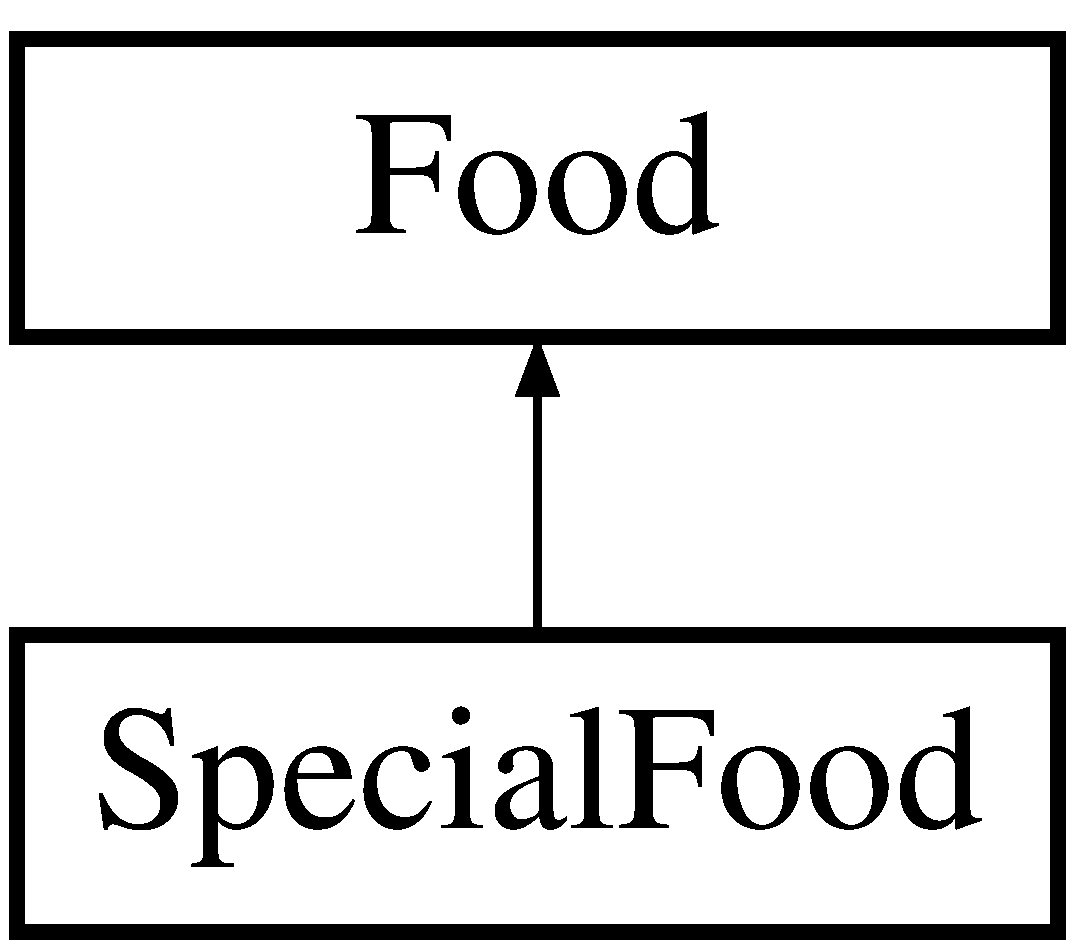
\includegraphics[height=2.000000cm]{classSpecialFood}
\end{center}
\end{figure}
\subsection*{\-Public \-Member \-Functions}
\begin{DoxyCompactItemize}
\item 
\hyperlink{classSpecialFood_af5257634148eee6b3b5f78b176f50a69}{\-Special\-Food} ()
\item 
\hyperlink{classSpecialFood_a189948b86e53cd790d1ed7be5f9325b9}{$\sim$\-Special\-Food} ()
\end{DoxyCompactItemize}


\subsection{\-Detailed \-Description}
\-A \hyperlink{classSpecialFood}{\-Special\-Food} piece \-A daughter of the \hyperlink{classFood}{\-Food} class. \-Represents a \-Windows 8 \-Logo. \-If \hyperlink{classSnake}{\-Snake} collides with \hyperlink{classSpecialFood}{\-Special\-Food}, a special game over will occur (\-B\-S\-O\-D). 

\subsection{\-Constructor \& \-Destructor \-Documentation}
\hypertarget{classSpecialFood_af5257634148eee6b3b5f78b176f50a69}{\index{\-Special\-Food@{\-Special\-Food}!\-Special\-Food@{\-Special\-Food}}
\index{\-Special\-Food@{\-Special\-Food}!SpecialFood@{\-Special\-Food}}
\subsubsection[{\-Special\-Food}]{\setlength{\rightskip}{0pt plus 5cm}{\bf \-Special\-Food\-::\-Special\-Food} (
\begin{DoxyParamCaption}
{}
\end{DoxyParamCaption}
)}}\label{classSpecialFood_af5257634148eee6b3b5f78b176f50a69}
\-Class \-Constructor -\/ loads first image, moves to random location. \-Precondition\-: \-A new instance of game was created. \-Postcondition\-: \-A new piece of food is created with \-Windows 8 logo image. \hypertarget{classSpecialFood_a189948b86e53cd790d1ed7be5f9325b9}{\index{\-Special\-Food@{\-Special\-Food}!$\sim$\-Special\-Food@{$\sim$\-Special\-Food}}
\index{$\sim$\-Special\-Food@{$\sim$\-Special\-Food}!SpecialFood@{\-Special\-Food}}
\subsubsection[{$\sim$\-Special\-Food}]{\setlength{\rightskip}{0pt plus 5cm}{\bf \-Special\-Food\-::$\sim$\-Special\-Food} (
\begin{DoxyParamCaption}
{}
\end{DoxyParamCaption}
)}}\label{classSpecialFood_a189948b86e53cd790d1ed7be5f9325b9}
\-Class \-Destructor -\/ \-Does \-Nothing 

\-The documentation for this class was generated from the following files\-:\begin{DoxyCompactItemize}
\item 
\hyperlink{SpecialFood_8h}{\-Special\-Food.\-h}\item 
\hyperlink{SpecialFood_8cpp}{\-Special\-Food.\-cpp}\end{DoxyCompactItemize}

\chapter{\-File \-Documentation}
\hypertarget{Food_8cpp}{\section{\-Food.\-cpp \-File \-Reference}
\label{Food_8cpp}\index{\-Food.\-cpp@{\-Food.\-cpp}}
}


\-Represents a \hyperlink{classFood}{\-Food} piece.  


{\ttfamily \#include \char`\"{}\-Food.\-h\char`\"{}}\*


\subsection{\-Detailed \-Description}
\-Represents a \hyperlink{classFood}{\-Food} piece. \begin{DoxyAuthor}{\-Author}
\-Chad \-Martin
\end{DoxyAuthor}
\-The parent of all food pieces. \-If not inherited, \hyperlink{classFood}{\-Food} represents a red or green \-Apple \-Logo. 
\hypertarget{Food_8h}{\section{\-Food.\-h \-File \-Reference}
\label{Food_8h}\index{\-Food.\-h@{\-Food.\-h}}
}


\-Represents a \hyperlink{classFood}{\-Food} piece.  


{\ttfamily \#include $<$\-Q\-Image$>$}\*
{\ttfamily \#include $<$\-Q\-Rect$>$}\*
{\ttfamily \#include $<$stdlib.\-h$>$}\*
\subsection*{\-Classes}
\begin{DoxyCompactItemize}
\item 
class \hyperlink{classFood}{\-Food}
\begin{DoxyCompactList}\small\item\em \-A \hyperlink{classFood}{\-Food} piece \-The parent of all food pieces. \-If not inherited, \hyperlink{classFood}{\-Food} represents a red or green \-Apple \-Logo. \end{DoxyCompactList}\end{DoxyCompactItemize}


\subsection{\-Detailed \-Description}
\-Represents a \hyperlink{classFood}{\-Food} piece. \begin{DoxyAuthor}{\-Author}
\-Chad \-Martin
\end{DoxyAuthor}
\-The parent of all food pieces. \-If not inherited, \hyperlink{classFood}{\-Food} represents a red or green \-Apple \-Logo. 
\hypertarget{FoodWinner_8cpp}{\section{\-Food\-Winner.\-cpp \-File \-Reference}
\label{FoodWinner_8cpp}\index{\-Food\-Winner.\-cpp@{\-Food\-Winner.\-cpp}}
}


\-Represents a \hyperlink{classFoodWinner}{\-Food\-Winner} piece.  


{\ttfamily \#include \char`\"{}\-Food\-Winner.\-h\char`\"{}}\*


\subsection{\-Detailed \-Description}
\-Represents a \hyperlink{classFoodWinner}{\-Food\-Winner} piece. \begin{DoxyAuthor}{\-Author}
\-Chad \-Martin
\end{DoxyAuthor}
\-A daughter of the \hyperlink{classFood}{\-Food} class. \-Represents a \-Linux \-Logo. \-If \hyperlink{classSnake}{\-Snake} collides with \hyperlink{classFoodWinner}{\-Food\-Winner}, a victory screen will occur. 
\hypertarget{FoodWinner_8h}{\section{\-Food\-Winner.\-h \-File \-Reference}
\label{FoodWinner_8h}\index{\-Food\-Winner.\-h@{\-Food\-Winner.\-h}}
}


\-Represents a \hyperlink{classFoodWinner}{\-Food\-Winner} piece.  


{\ttfamily \#include \char`\"{}\-Food.\-h\char`\"{}}\*
{\ttfamily \#include $<$\-Q\-Image$>$}\*
{\ttfamily \#include $<$\-Q\-Rect$>$}\*
\subsection*{\-Classes}
\begin{DoxyCompactItemize}
\item 
class \hyperlink{classFoodWinner}{\-Food\-Winner}
\begin{DoxyCompactList}\small\item\em \-A \hyperlink{classFoodWinner}{\-Food\-Winner} piece \-A daughter of the \hyperlink{classFood}{\-Food} class. \-Represents a \-Linux \-Logo. \-If \hyperlink{classSnake}{\-Snake} collides with \hyperlink{classFoodWinner}{\-Food\-Winner}, a victory screen will occur. \end{DoxyCompactList}\end{DoxyCompactItemize}


\subsection{\-Detailed \-Description}
\-Represents a \hyperlink{classFoodWinner}{\-Food\-Winner} piece. \begin{DoxyAuthor}{\-Author}
\-Chad \-Martin
\end{DoxyAuthor}
\-A daughter of the \hyperlink{classFood}{\-Food} class. \-Represents a \-Linux \-Logo. \-If \hyperlink{classSnake}{\-Snake} collides with \hyperlink{classFoodWinner}{\-Food\-Winner}, a victory screen will occur. 
\hypertarget{Game_8cpp}{\section{\-Game.\-cpp \-File \-Reference}
\label{Game_8cpp}\index{\-Game.\-cpp@{\-Game.\-cpp}}
}


\-Contians the \hyperlink{classSnake}{\-Snake} \hyperlink{classGame}{\-Game} \-Logic.  


{\ttfamily \#include \char`\"{}\-Game.\-h\char`\"{}}\*
{\ttfamily \#include $<$\-Q\-Painter$>$}\*
{\ttfamily \#include $<$\-Q\-Application$>$}\*


\subsection{\-Detailed \-Description}
\-Contians the \hyperlink{classSnake}{\-Snake} \hyperlink{classGame}{\-Game} \-Logic. \begin{DoxyAuthor}{\-Author}
\-Chad \-Martin
\end{DoxyAuthor}
\-This class contains the logic that makes up the \hyperlink{classSnake}{\-Snake} \hyperlink{classGame}{\-Game}. 
\hypertarget{Game_8h}{\section{\-Game.\-h \-File \-Reference}
\label{Game_8h}\index{\-Game.\-h@{\-Game.\-h}}
}


\-Contians the \hyperlink{classSnake}{\-Snake} \hyperlink{classGame}{\-Game} \-Logic.  


{\ttfamily \#include \char`\"{}\-Snake\-Block.\-h\char`\"{}}\*
{\ttfamily \#include \char`\"{}\-Snake.\-h\char`\"{}}\*
{\ttfamily \#include \char`\"{}\-Food.\-h\char`\"{}}\*
{\ttfamily \#include \char`\"{}\-Special\-Food.\-h\char`\"{}}\*
{\ttfamily \#include \char`\"{}\-Food\-Winner.\-h\char`\"{}}\*
{\ttfamily \#include \char`\"{}iphone.\-h\char`\"{}}\*
{\ttfamily \#include $<$vector$>$}\*
{\ttfamily \#include $<$\-Q\-Widget$>$}\*
{\ttfamily \#include $<$\-Q\-Key\-Event$>$}\*
\subsection*{\-Classes}
\begin{DoxyCompactItemize}
\item 
class \hyperlink{classGame}{\-Game}
\begin{DoxyCompactList}\small\item\em \-The \hyperlink{classSnake}{\-Snake} \hyperlink{classGame}{\-Game} \-Logic. \-This class contains the logic that makes up the \hyperlink{classSnake}{\-Snake} \hyperlink{classGame}{\-Game}. \end{DoxyCompactList}\end{DoxyCompactItemize}


\subsection{\-Detailed \-Description}
\-Contians the \hyperlink{classSnake}{\-Snake} \hyperlink{classGame}{\-Game} \-Logic. \begin{DoxyAuthor}{\-Author}
\-Chad \-Martin
\end{DoxyAuthor}
\-This class contains the logic that makes up the \hyperlink{classSnake}{\-Snake} \hyperlink{classGame}{\-Game}. 
\hypertarget{iphone_8cpp}{\section{iphone.\-cpp \-File \-Reference}
\label{iphone_8cpp}\index{iphone.\-cpp@{iphone.\-cpp}}
}


\-Contains \hyperlink{classIphone}{\-Iphone} image and location.  


{\ttfamily \#include \char`\"{}iphone.\-h\char`\"{}}\*


\subsection{\-Detailed \-Description}
\-Contains \hyperlink{classIphone}{\-Iphone} image and location. \begin{DoxyAuthor}{\-Author}
\-Chad \-Martin
\end{DoxyAuthor}
\-A \hyperlink{classIphone}{\-Iphone} image and location of where to paint. 
\hypertarget{iphone_8h}{\section{iphone.\-h \-File \-Reference}
\label{iphone_8h}\index{iphone.\-h@{iphone.\-h}}
}


\-Contains \hyperlink{classIphone}{\-Iphone} image and location.  


{\ttfamily \#include $<$\-Q\-Image$>$}\*
{\ttfamily \#include $<$\-Q\-Rect$>$}\*
\subsection*{\-Classes}
\begin{DoxyCompactItemize}
\item 
class \hyperlink{classIphone}{\-Iphone}
\begin{DoxyCompactList}\small\item\em \-A \hyperlink{classIphone}{\-Iphone} image and location of where to paint. \end{DoxyCompactList}\end{DoxyCompactItemize}


\subsection{\-Detailed \-Description}
\-Contains \hyperlink{classIphone}{\-Iphone} image and location. \begin{DoxyAuthor}{\-Author}
\-Chad \-Martin
\end{DoxyAuthor}
\-A \hyperlink{classIphone}{\-Iphone} image and location of where to paint. 
\hypertarget{main_8cpp}{\section{main.\-cpp \-File \-Reference}
\label{main_8cpp}\index{main.\-cpp@{main.\-cpp}}
}


\-Contians \-Main function which initializes \hyperlink{classGame}{\-Game} object.  


{\ttfamily \#include \char`\"{}\-Game.\-h\char`\"{}}\*
{\ttfamily \#include $<$\-Q\-Desktop\-Widget$>$}\*
{\ttfamily \#include $<$\-Q\-Application$>$}\*
\subsection*{\-Functions}
\begin{DoxyCompactItemize}
\item 
void \hyperlink{main_8cpp_a9249374e4101a15aa94e470ac81bcf46}{center} (\-Q\-Widget \&widget)
\begin{DoxyCompactList}\small\item\em \-Sets up window size and centers window on screen. \-Precondition\-: \-Program has started. \-Postcondition\-: \hyperlink{classGame}{\-Game} window is displayed on center of screen. \end{DoxyCompactList}\item 
\hypertarget{main_8cpp_a0ddf1224851353fc92bfbff6f499fa97}{int {\bfseries main} (int argc, char $\ast$argv\mbox{[}$\,$\mbox{]})}\label{main_8cpp_a0ddf1224851353fc92bfbff6f499fa97}

\end{DoxyCompactItemize}


\subsection{\-Detailed \-Description}
\-Contians \-Main function which initializes \hyperlink{classGame}{\-Game} object. \begin{DoxyAuthor}{\-Author}
\-Chad \-Martin
\end{DoxyAuthor}
\-This file is used to generate and set up a window for the game snake to be played in. 

\subsection{\-Function \-Documentation}
\hypertarget{main_8cpp_a9249374e4101a15aa94e470ac81bcf46}{\index{main.\-cpp@{main.\-cpp}!center@{center}}
\index{center@{center}!main.cpp@{main.\-cpp}}
\subsubsection[{center}]{\setlength{\rightskip}{0pt plus 5cm}void {\bf center} (
\begin{DoxyParamCaption}
\item[{\-Q\-Widget \&}]{widget}
\end{DoxyParamCaption}
)}}\label{main_8cpp_a9249374e4101a15aa94e470ac81bcf46}


\-Sets up window size and centers window on screen. \-Precondition\-: \-Program has started. \-Postcondition\-: \hyperlink{classGame}{\-Game} window is displayed on center of screen. 


\begin{DoxyParams}{\-Parameters}
{\em \&widget} & \-A user interface object. \\
\hline
\end{DoxyParams}

\hypertarget{mainpage_8h}{\section{mainpage.\-h \-File \-Reference}
\label{mainpage_8h}\index{mainpage.\-h@{mainpage.\-h}}
}


\-Contains main \-Page documentation.  




\subsection{\-Detailed \-Description}
\-Contains main \-Page documentation. \begin{DoxyAuthor}{\-Author}
\-Chad \-Martin 
\end{DoxyAuthor}

\hypertarget{Snake_8cpp}{\section{\-Snake.\-cpp \-File \-Reference}
\label{Snake_8cpp}\index{\-Snake.\-cpp@{\-Snake.\-cpp}}
}


\-Represents the infinitely growing \hyperlink{classSnake}{\-Snake}.  


{\ttfamily \#include \char`\"{}\-Snake.\-h\char`\"{}}\*


\subsection{\-Detailed \-Description}
\-Represents the infinitely growing \hyperlink{classSnake}{\-Snake}. \begin{DoxyAuthor}{\-Author}
\-Chad \-Martin
\end{DoxyAuthor}
\-This class represents the infinitely growing snake which is made up of a vector of \hyperlink{classSnakeBlock}{\-Snake\-Block} pointers. 
\hypertarget{Snake_8h}{\section{\-Snake.\-h \-File \-Reference}
\label{Snake_8h}\index{\-Snake.\-h@{\-Snake.\-h}}
}


\-Represents the infinitely growing \hyperlink{classSnake}{\-Snake}.  


{\ttfamily \#include $<$\-Q\-Image$>$}\*
{\ttfamily \#include $<$\-Q\-Rect$>$}\*
{\ttfamily \#include $<$\-Q\-Painter$>$}\*
{\ttfamily \#include $<$vector$>$}\*
{\ttfamily \#include \char`\"{}\-Snake\-Block.\-h\char`\"{}}\*
{\ttfamily \#include \char`\"{}\-Food.\-h\char`\"{}}\*
\subsection*{\-Classes}
\begin{DoxyCompactItemize}
\item 
class \hyperlink{classSnake}{\-Snake}
\begin{DoxyCompactList}\small\item\em \-The \hyperlink{classSnake}{\-Snake} \-Represents the infinitely growing snake which is made up of a vector of \hyperlink{classSnakeBlock}{\-Snake\-Block} pointers. \end{DoxyCompactList}\end{DoxyCompactItemize}


\subsection{\-Detailed \-Description}
\-Represents the infinitely growing \hyperlink{classSnake}{\-Snake}. \begin{DoxyAuthor}{\-Author}
\-Chad \-Martin
\end{DoxyAuthor}
\-This class represents the infinitely growing snake which is made up of a vector of \hyperlink{classSnakeBlock}{\-Snake\-Block} pointers. 
\hypertarget{SnakeBlock_8cpp}{\section{\-Snake\-Block.\-cpp \-File \-Reference}
\label{SnakeBlock_8cpp}\index{\-Snake\-Block.\-cpp@{\-Snake\-Block.\-cpp}}
}


\-Represents the \hyperlink{classSnakeBlock}{\-Snake\-Block}.  


{\ttfamily \#include \char`\"{}\-Snake\-Block.\-h\char`\"{}}\*


\subsection{\-Detailed \-Description}
\-Represents the \hyperlink{classSnakeBlock}{\-Snake\-Block}. \begin{DoxyAuthor}{\-Author}
\-Chad \-Martin
\end{DoxyAuthor}
\-This class represents one block of the \hyperlink{classSnake}{\-Snake}. 
\hypertarget{SnakeBlock_8h}{\section{\-Snake\-Block.\-h \-File \-Reference}
\label{SnakeBlock_8h}\index{\-Snake\-Block.\-h@{\-Snake\-Block.\-h}}
}


\-Represents the \hyperlink{classSnakeBlock}{\-Snake\-Block}.  


{\ttfamily \#include $<$\-Q\-Image$>$}\*
{\ttfamily \#include $<$\-Q\-Rect$>$}\*
\subsection*{\-Classes}
\begin{DoxyCompactItemize}
\item 
class \hyperlink{classSnakeBlock}{\-Snake\-Block}
\begin{DoxyCompactList}\small\item\em \-The \hyperlink{classSnakeBlock}{\-Snake\-Block} \-Represents one block of the \hyperlink{classSnake}{\-Snake}. \end{DoxyCompactList}\end{DoxyCompactItemize}


\subsection{\-Detailed \-Description}
\-Represents the \hyperlink{classSnakeBlock}{\-Snake\-Block}. \begin{DoxyAuthor}{\-Author}
\-Chad \-Martin
\end{DoxyAuthor}
\-This class represents one block of the \hyperlink{classSnake}{\-Snake}. 
\hypertarget{SpecialFood_8cpp}{\section{\-Special\-Food.\-cpp \-File \-Reference}
\label{SpecialFood_8cpp}\index{\-Special\-Food.\-cpp@{\-Special\-Food.\-cpp}}
}


\-Represents a \hyperlink{classSpecialFood}{\-Special\-Food} piece.  


{\ttfamily \#include \char`\"{}\-Special\-Food.\-h\char`\"{}}\*


\subsection{\-Detailed \-Description}
\-Represents a \hyperlink{classSpecialFood}{\-Special\-Food} piece. \begin{DoxyAuthor}{\-Author}
\-Chad \-Martin
\end{DoxyAuthor}
\-A daughter of the \hyperlink{classFood}{\-Food} class. \-Represents a \-Windows 8 \-Logo. \-If \hyperlink{classSnake}{\-Snake} collides with \hyperlink{classSpecialFood}{\-Special\-Food}, a special game over will occur (\-B\-S\-O\-D). 
\hypertarget{SpecialFood_8h}{\section{\-Special\-Food.\-h \-File \-Reference}
\label{SpecialFood_8h}\index{\-Special\-Food.\-h@{\-Special\-Food.\-h}}
}


\-Represents a \hyperlink{classSpecialFood}{\-Special\-Food} piece.  


{\ttfamily \#include \char`\"{}\-Food.\-h\char`\"{}}\*
{\ttfamily \#include $<$\-Q\-Image$>$}\*
{\ttfamily \#include $<$\-Q\-Rect$>$}\*
\subsection*{\-Classes}
\begin{DoxyCompactItemize}
\item 
class \hyperlink{classSpecialFood}{\-Special\-Food}
\begin{DoxyCompactList}\small\item\em \-A \hyperlink{classSpecialFood}{\-Special\-Food} piece \-A daughter of the \hyperlink{classFood}{\-Food} class. \-Represents a \-Windows 8 \-Logo. \-If \hyperlink{classSnake}{\-Snake} collides with \hyperlink{classSpecialFood}{\-Special\-Food}, a special game over will occur (\-B\-S\-O\-D). \end{DoxyCompactList}\end{DoxyCompactItemize}


\subsection{\-Detailed \-Description}
\-Represents a \hyperlink{classSpecialFood}{\-Special\-Food} piece. \begin{DoxyAuthor}{\-Author}
\-Chad \-Martin
\end{DoxyAuthor}
\-A daughter of the \hyperlink{classFood}{\-Food} class. \-Represents a \-Windows 8 \-Logo. \-If \hyperlink{classSnake}{\-Snake} collides with \hyperlink{classSpecialFood}{\-Special\-Food}, a special game over will occur (\-B\-S\-O\-D). 
\printindex
\end{document}
